%for a more compact document, add the option openany to avoid
%starting all chapters on odd numbered pages
\documentclass[12pt]{cmuthesis}

% This is a template for a CMU thesis.  It is 18 pages without any content :-)
% The source for this is pulled from a variety of sources and people.
% Here's a partial list of people who may or may have not contributed:
%
%        bnoble   = Brian Noble
%        caruana  = Rich Caruana
%        colohan  = Chris Colohan
%        jab      = Justin Boyan
%        josullvn = Joseph O'Sullivan
%        jrs      = Jonathan Shewchuk
%        kosak    = Corey Kosak
%        mjz      = Matt Zekauskas (mattz@cs)
%        pdinda   = Peter Dinda
%        pfr      = Patrick Riley
%        dkoes = David Koes (me)

% My main contribution is putting everything into a single class files and small
% template since I prefer this to some complicated sprawling directory tree with
% makefiles.

% some useful packages
\usepackage{subcaption}
\usepackage{times}
\usepackage{fullpage}
\usepackage{graphicx}
\usepackage{amsmath}
\usepackage{titlesec}
\usepackage{amsfonts}
\usepackage{tikz}
\usepackage{wrapfig}
\usepackage{lettrine}
\usepackage{algorithm2e}
\usepackage{multirow}
\usepackage{booktabs}
\usepackage{wrapfig}
\usetikzlibrary{bayesnet}
\usetikzlibrary{shapes,arrows}
\usepackage[numbers,sort]{natbib}
\usepackage[backref,pageanchor=true,plainpages=false, pdfpagelabels, bookmarks,bookmarksnumbered,
%pdfborder=0 0 0,  %removes outlines around hyper links in online display
]{hyperref}

% Approximately 1" margins, more space on binding side
%\usepackage[letterpaper,twoside,vscale=.8,hscale=.75,nomarginpar]{geometry}
%for general printing (not binding)
\usepackage[letterpaper,twoside,vscale=.8,hscale=.75,nomarginpar,hmarginratio=1:1]{geometry}

% Provides a draft mark at the top of the document. 
\draftstamp{\today}{DRAFT}
 
\titleformat{\chapter}[display]{\normalfont\Large}{\textsc{Chapter \thechapter~~}}{0pt}{\Huge}
\titleformat{\section}[hang]{\normalfont\itshape\Large}{\thesection~~}{0pt}{\Large}
\titleformat{\subsection}[hang]{\normalfont\large}{\thesubsection~~}{0pt}{\large}

\newcommand{\blankpage}{\newpage\hbox{}\thispagestyle{empty}\newpage} % Command to insert a blank page
\newcommand{\apriori}{\textit{a. priori}}
\newcommand{\eg}{\textit{e.g.}}
\newcommand{\ie}{\textit{i.e.}}
\newcommand{\argmin}{\operatornamewithlimits{argmin}}
\newcommand{\argmax}{\operatornamewithlimits{argmax}}
\newcommand{\subsectionbf}[1]{\subsection{\textbf{#1}}}
\newcommand{\sectionbf}[1]{\section{\textbf{#1}}}
\newcommand{\figref}[1]{Fig.~\ref{#1}~}
\newcommand{\tableref}[1]{Table ~\ref{#1}~}
\newcommand{\sref}[1]{{see page~\pageref{#1}}}
\newcommand{\eqnref}[1]{Eq.~\ref{#1}~}
\newcommand{\algref}[1]{Alg.~\ref{#1}~}
\newcommand{\Prob}{\text{P}}
\newcommand{\Expec}{\text{E}}
\newcommand{\qvec}{\mathbf{q}}
\newcommand{\uvec}{\mathbf{u}}
\newcommand{\xvec}{\mathbf{x}}
\newcommand{\Proj}{\pi}
\newcommand{\InvProj}{\text{Proj}^{-1}}
\newcommand{\Q}{\mathbf{Q}}
\newcommand{\R}{\mathbb{R}}
\newcommand{\ROne}{\R}
\newcommand{\RTwo}{\R^2}
\newcommand{\RThree}{\R^3}
\newcommand{\RN}{\R^N}
\newcommand{\SEThree}{SE(3)}
\newcommand{\SOThree}{SO(3)}
\newcommand{\config}{\qvec}
\newcommand{\inv}{^{-1}}
\newcommand{\J}{\mathbf{J}}
\newcommand{\trans}{^{T}}
\newcommand{\Imagespace}{\Omega}
\newcommand{\Image}{\mathbf{I}}
\newcommand{\DepthImage}{\mathbf{D}}
\newcommand{\eye}{\mathbf{I}}
\newcommand{\pixel}{\mathbf{p}}
\newcommand{\enc}{\theta}
\newcommand{\DenseMap}{\mathbf{M}}
\newcommand{\SparseMap}{\mathbf{M}}
\newcommand{\Extr}{K_\text{cam}}
\newcommand{\landmark}{\mathbf{l}}
\newcommand{\measurement}{\mathbf{z}}
\newcount\colveccount
\newcommand*\colvec[1]{
        \global\colveccount#1
        \begin{bmatrix}
        \colvecnext
}
\def\colvecnext#1{
        #1
        \global\advance\colveccount-1
        \ifnum\colveccount>0
                \\
                \expandafter\colvecnext
        \else
                \end{bmatrix}
        \fi
}
 
 
\begin {document} 
\frontmatter

%initialize page style, so contents come out right (see bot) -mjz
\pagestyle{empty}
 
\title{ {\bf Tracking and Calibrating Articulated Robots using SLAM Techniques}}
\author{Matthew Klingensmith}
\date{\today}
\trnumber{}

\committee{
Siddhartha S. Srinivasa  \\
Michael Kaess  \\
George Kantor \\
Andrew Davison 
}

\support{Work in this disseration was supported in part by Toyota USA grant No. 1011344 the U.S Office of Naval Research grant No. N000141210613 and NSF grant No. IIS-1426703}
\disclaimer{}

% copyright notice generated automatically from Year and author.
% permission added if \permission{} given.

\keywords{SLAM, Calibration, Tracking, Kinematics, Manipulation, Visual Servoing, Computer Vision, 3D Mapping}

\maketitle 

\begin{dedication}
For my parents, who showed me the way; \\
Sarah, who lit up my life; \\
and David, who still haunts me.
\end{dedication}

\pagestyle{plain} % for toc, was empty

%% Obviously, it's probably a good idea to break the various sections of your thesis
%% into different files and input them into this file...

\begin{abstract}
%
\end{abstract}

\begin{acknowledgments}
%
\end{acknowledgments}

\tableofcontents
\listoffigures
\listoftables

\mainmatter

%% Double space document for easy review:
%\renewcommand{\baselinestretch}{1.66}\normalsize
%\chapter*{Foreward} I have been working with robot manipulators for quite a while now. One of the things that has surprised me most about robots is their almost unbelievable incompetence. Popular science fiction led me to believe that robots would have superhuman abilities. 

To be fair, many robots \textit{really are} superhuman. Just look at any factory floor. These days, factories (especially car factories) are filled with huge, lumbering industrial robots that do the same tasks again and again at breakneck speeds -- welding, lifting huge loads, bending metal, and precisely placing tiny parts. That's something I couldn't do with my measly human hands and brain even in principle.

But in spite of their obvious advantages, industrial robots have an embarassing secret: for the most part, they're programmed in an ad-hoc matter by hand, and follow their programming without question. You might notice that on the factory floor, the robots are in cages, and there aren't any people around. This is because when you've got a 4-ton robot moving around at breakneck speeds according to a rigid program, it doesn't play nicely with any human beings that might be standing in the way. You might also notice that in factories, each robot performs an extremely well-defined task (such as screwing in four specific bolts, or spraying paint at one specific part of a specific kind of car chassis). The sad matter of fact is, if the task that the industrial robot has to perform were to change only slightly, its program would fail spectacularly.

In undergrad, as part of a manipulation class we programmed an ABB industrial robot to pick highlighters out of a box in Matt Mason's lab, and show them to a camera. It was supposed to pick thousands of these things out of the bin to train a machine learning algorithm. The robot was using simple position control to move about. It would drop the markers on a styrofoam ramp, whcih would then slide back into the bin. At a rate of about one highlighter every twenty seconds, it would take many hours to train the system. While waiting for the robot to complete its task, I fell asleep on the couch in the lab. A couple of hours later, I was awoken by a loud \textit{crash}. Somehow, the robot had smashed the ramp to bits, and was presently dropping markers onto the floor as if nothing had happened. That's not exactly superhuman performance.

As you might guess, robots need to be a lot smarter to tackle real-world tasks, where things are constantly changing and you can't afford to be so rigid. That means taking in information from sensing, detecting failure, and coming up with new plans of action as tasks change. As humans, we take these things for granted. Even the youngest babies are capable of reacting to changes in their environments, and next to industrial robots look like geniuses when it comes to manipulating novel objects. Robotics research is all about making this kind of baby-like performance possible. The holy grail of robotic manipulation would be a system that could adapt as quickly as a newborn. This phenomenon (sometimes called \textit{Moravec's Paradox}, after Hans Moravec, the famous CMU roboticist) haunts robotics. Humans think manipulation is easy because we were quite literally born to manipulate. We are like natural-born piano virtuous who glibly declare that piano playing is easy, and all it takes is a bit of intuition.

I witnessed several other instances of robotic incompetence during the DARPA ARM-S challenge. The idea behind the challenge was that teams of manipulation experts from universities around the world would program a robot to autonomously complete some ``simple'' manipulation tasks such as picking up objects, using simple tools, opening doors, etc. I was lucky enough to work as a student intern and later as a software engineer on this multi-year project for the team at NREC. If I was to describe our team's initial strategy with one word, it would be \textit{modularity}. We broke the problem of grasping down into a few simple steps described in the literature as the ``grasping pipeline'' (\figref{fig:grasp_pipeline}).

\begin{figure}
\centering
	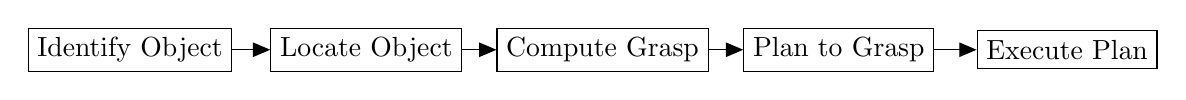
\begin{tikzpicture}
		\node[draw] (ident) at (0, 0) {Identify Object};
		\node[draw] (locate) at (3, 0) {Locate Object};
		\node[draw] (plan_grasp) at (6, 0) {Compute Grasp};
		\node[draw] (motion_plan) at (9, 0) {Plan to Grasp};
		\node[draw] (close) at (11.9, 0) {Execute Plan};
		\path [draw, ->] (ident) -- (locate);
		\path [draw, ->] (locate) -- (plan_grasp);
		\path [draw, ->] (plan_grasp) -- (motion_plan);
		\path [draw, ->] (motion_plan) -- (close);
	\end{tikzpicture}
\caption{The so-called grasping pipeline.}
\label{fig:grasp_pipeline}
\end{figure}

The idea behind the grasping pipeline is that the ``perception people'' can simply work on the first two steps (identifying and locating objects), the ``planning people'' can work on on the third and fourth steps (determining how to grasp a known object and how to exectue that grasp), and finally the ``controls people'' can focus on the final step, which is actually executing the plan that was passed to them. 

In this context, each module is just a black box with well-defined inputs and outputs. As specialists, we like such black boxes because they allow us to keep the messy bits of the other guy's box out of our mind and focus on solving the problem. The perception people never need to ask ``how will uncertainty in my perception system affect the grasp planner?'' the planning people never have to ask ``what if the execution fails?'' and the execution people never have to ask ``what do I do if the plan is wrong?''

Of course, when we strung all the black boxes together, we got a result that was less than satisfactory. Very often, the robot's beautiful grasp plan would put it a few millimeters away from where it was supposed to be, the fingers would close, and the grasp would fail completely. 

Why does this happen? In a word: \textit{uncertainty}. The perception system didn't know exactly where the objects were. The robot's model of its own kinematics were not exactly correct. The controller was noisy and didn't perfectly follow the planner's trajectory. Ultimately, the boxes were not supposed to be so black. The perception system should have detected that the robot wasn't where it was supposed to be, the planning system should have generated a new plan of action when this was detected, and the execution system should have responded to the new plans. In other words, \textit{Moravec's Paradox} had reared its ugly head in our system design, making it far too optimistically simple.

By the end of the challenge, our system design had changed to something much more complex and robust. The core of our design shifted from \textit{planning} to \textit{control}. We had a perception system that fed data directly into the controller, which directly adjusted according to changes in the environment. 

In my opinion, the critical bit of engineering that changed our grasping pipeline from something embarassing to something workable was 3D visual servoing. The idea behind 3D visual servoing is quite simple: you perceive the robot and its goal, figure out how much error there is between the current state of the robot and where you want it to be, and then you tell the controller to take a step toward reducing the error. This strategy has a beautiful simplicitly which naturally reduces uncertainty. Errors in the robot's kinematics, object sensing, and control are all forced into the same reference frame, where small corrections can be made to reduce them. 

This is far better than trying to correct all the error beforehand using calibration and then blindly trying to execute a plan with the faith that your calibration is perfect. In fact, our servoing allowed us to be lazy. We hardly ever recalibrated the robot's joint encoders or camera extrinsics -- the visual servoing made all of that unnecessary.

This thesis is about developing systems which use perception in the loop with a robot arm to correct error in its calibration. The first section is about work I did with ARM-S on tracking the robot arm with an external depth camera, which was a critical component in our visual servoing architecture. The second section takes the same idea and extends it to a hand-mounted depth camera which cannot see any part of the robot. This was done for the ADA project at the Personal Robotics Lab. The third section generalizes this idea to a SLAM framework which can support multiple sensor types, calibration parameters, and uncertainty models; which I developed while visiting the Dyson Robotics Lab at Imperial College London.

My hope is that the research I present here will help elucidate some of the challenges of properly calibrating and tracking robots online, and how some general techniques from computer vision and SLAM can be used for this purpose.
\chapter{Introduction} \input{intro} 
\chapter{Dense Tracking with an External Depth Sensor} \label{chap:dense_external_tracking}
\begin{figure}
	\begin{center}
		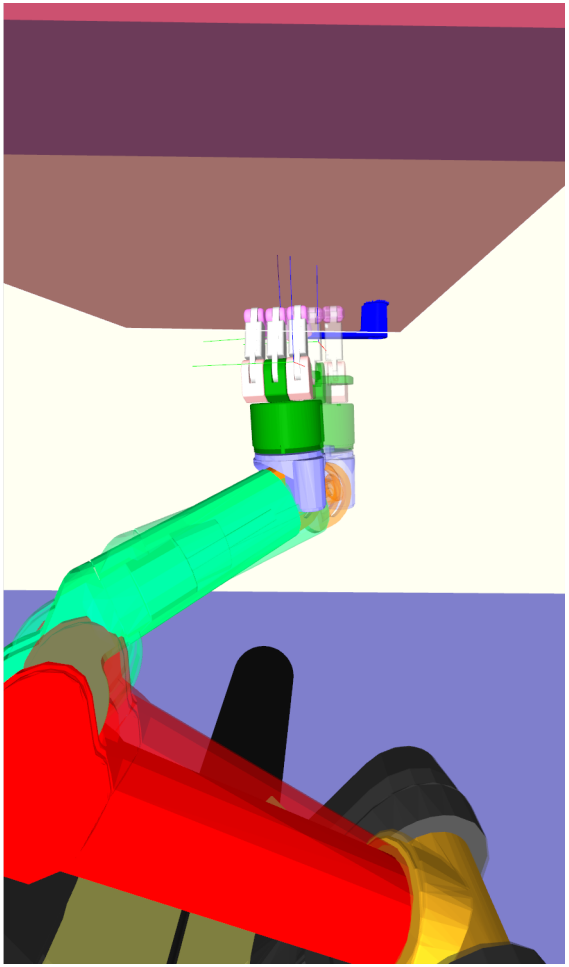
\includegraphics[width=0.24\textwidth]{img/dense_tracking/door_sim}
		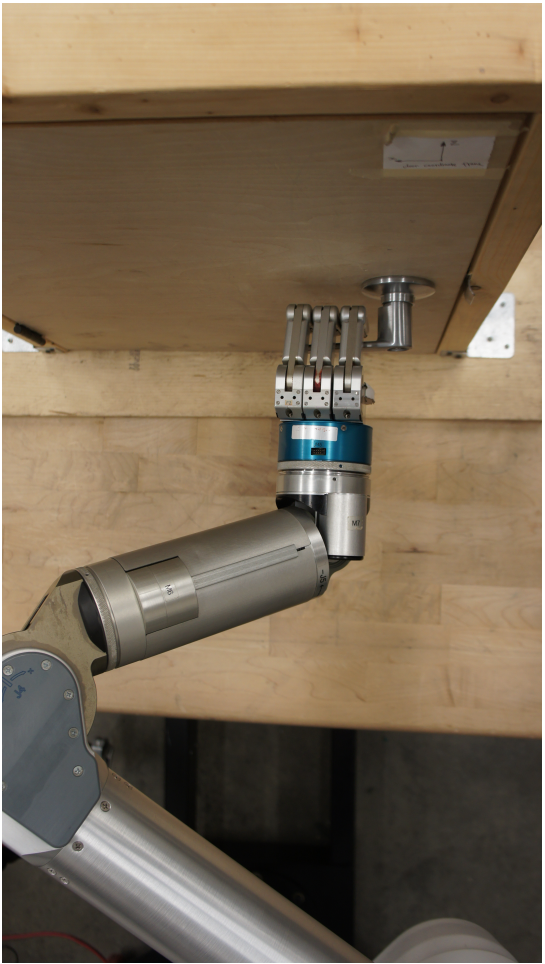
\includegraphics[width=0.23\textwidth]{img/dense_tracking/door_real}
	\end{center}
	\caption{A robot arm opens a door using dense depth tracking. Left: the robot's kinematics (solid) are compared with the estimated joint angles from the tracking system (transparent). Right: the robot is shown grasping the door handle.}
	\label{fig:door_open}
\end{figure}
\lettrine{W}e first consider the case of using an external depth camera to track a noisy robot arm in real time. In this case, a depth sensor is mounted so that it can see all or part of the robot's arm, and the robot's joint angles are estimated from the depth image. This is the simplest of the three problems we will consider, because we generally have a good 3D model of the robot arm, and this model can be used as the basis of a tracking algorithm. 

Tracking the arm in real-time also allows for a kind of 3D visual servoing, where the robot can be made to touch points in the scene while automatically correcting for its joint angle error. This rather powerful technique allows the robot to correct unforseen errors that arise from its own dynamics, contact with the scene, and more. In addition, solving this problem elucidates the structure of the related problems we will have to solve in later sections. \footnote{\textit{This chapter largely reiterates earlier work that appears in \cite{Klingensmith2013}}} 

\section{Problem Definition}
We have a series of discrete time-steps $t_1 \ldots T$ in which we receive time-synchronized measurements from the encoders $\enc_1 \ldots \enc_T$ and depth images $D_1 \ldots D_T$. How do we determine the true state of the robot from these data? One approach might be to track a rigid object on the robot's body (such as its end effector); but this ignores valuable data from other parts of the robot's body. Another approach is to track the entire robot arm using the depth image.In this section, we will derive a simple way of tracking the entire robot in \textit{configuration space} (\sref{sec:articulated_linkage}) from a series of depth images. This has several advantages: it makes full use of observations of the robot's body, it naturally constrains solutions to those which are possible given the robot's kinematics, and it provides an estimate of the joint angles which can be used for visual servoing.

The goal is to predict a maximum likelihood estimate of the robot's true configuration $\config_1 \ldots \config_T$ from these measurements. In other words, we wish to find:

\begin{equation}
	\config_T = \argmax_{\config} \Prob\left(\config | \DepthImage_1, \ldots, \DepthImage_T, \enc_1, \ldots \enc_T \right)
\end{equation}

If we model this as a Markov process, such that the state at time $T$ only depends on the state at time $T - 1$ and measurements from time $T$, and assuming conditional independence between the depth image, configuration and joint encoders we have a maximization of the log-likehihood of two terms:

\begin{align}
	\config_T &= \argmax_{\config} \Prob\left(\config | \DepthImage_T, \enc_T\right) \\
	          &= \argmax_{\config} \frac{\Prob\left(\DepthImage_T | \config\right) \Prob(\config | \enc_T)}{\Prob\left(\DepthImage_T, \enc_T\right)} \\
	          &= \argmax_{\config} \log \Prob(\DepthImage_T | \config) + \log \Prob(\config | \enc_T)
	          \label{eqn:dense_model_track}
\end{align} 

\noindent these are the depth image posterior $\Prob(\DepthImage_T | \config)$ and the joint encoder posterior $\Prob(\config | \enc_T)$. With some simple assumptions about the structure of the depth image and the joint encoders, it is possible to write these out efficiently.

\subsection{Depth Image Posterior}
From each depth image $\DepthImage_T$, produce its point-cloud $\pixel_1, \ldots, \pixel_M \in \DepthImage_T$. We assume that given the robot's configuration $\config$, the points in the point cloud correspond to some true point on the robot's body corrupted by identically distributed indepdendent random noise. Assume there is a ground-truth mapping $\beta_i(\config)$ that gives us the point on the robot's body that corresponds to the point in the point cloud of the depth image.

Assume then that the points are distributed according to a simple isotropic normal distribution so that

\begin{equation}
	\pixel_i \sim \beta_i(\pixel_i, \config) + \mathcal{N}(0, \Sigma_\pixel)
\end{equation}

\noindent where $\Sigma_\pixel =  \sigma_\pixel \eye$ is the covariance of the point cloud noise, with $\sigma_\pixel$ being the noise variance. With all these assumptions in place, the probability of seeing a particular point in the point cloud given the robot's configuration is simply

\begin{equation}
	\Prob(\pixel_i | \config) = \exp{\frac{-\|\pixel_i - \beta_i(\config)\|^2}{2 \sigma_\pixel}}
\end{equation}

\noindent and assuming conditional independence, the depth image posterior becomes

\begin{equation}
	\Prob(\DepthImage_T | \config) = \prod_{\pixel_i \in \DepthImage_T} \Prob(\pixel_i | \config)
\end{equation}

\noindent and finally the log-likelihood becomes

\begin{equation}
	\log \Prob(\DepthImage_T | \config) = -\frac{1}{2 \sigma_\pixel}\sum_{\pixel_i \in \DepthImage_T} \| \pixel - \beta_i(\config) \|^2
\end{equation}

Computing the posterior requires associating each point in the point cloud with a point on the robot's body. If these associations are unknown, we can use physical distance as a heuristic to match a point in the point cloud to one on the robot's body. That is:

\begin{equation}
	\bar{\beta_i}(\config) = \argmin_{\beta \in \mathbf{B}(\config)} \|\beta - \pixel_i\|
\end{equation}

\noindent where $\mathbf{B}(\config)$ is the set of all points on the robot's body while the robot is in configuration $\config$ that can be viewed by the depth camera (and which are not self-occluded). This heuristic is similar to the one used in the Iterative Closest Point (ICP) algorithm. Because we use every pixel in the depth image, this is a \textit{dense} tracking technique (as opposed to a technique which only uses sparse image features).

\subsection{Joint Encoder Posterior}
The relationship between the joint encoders $\enc$ and actual configuration $\config$ of the robot might be quite complicated; but here we use a very simple model of the joint encoder noise that is sufficient to capture it. Assume we have a fixed calibration $K_\enc(\enc)$ which converts joint encoders to robot configurations (\sref{sec:encoders}), and assume that the true robot configuration is drawn from an isotropic gaussian distribution around this function. That is:

\begin{equation}
	\config_T \sim K_\enc(\enc_T) + \mathcal{N}(0, \Sigma_\config)
\end{equation}

\noindent where $\Sigma_\config = \sigma_\config \eye$, and  $\sigma_\config$ is the isotropic variance of the noise. With these assumptions, we can write the joint encoder posterior as

\begin{equation}
	\Prob(\config_T | \enc_T) = \exp{-\frac{\|K_\enc(\enc_T) - \config\|^2}{2 \sigma_\config}}
\end{equation} 

\noindent and the log-likelihood is simply

\begin{equation}
	\log P(\config_T | \enc_T) = -\frac{\|K_\enc(\enc_T) - \config\|^2}{2 \sigma_\config}
\end{equation}

\noindent admittedly, this model of joint encoder noise is not completely accurate, as it assumes there is time-independent random noise on the joint-encoders, when in reality there are likely to be systematic biases that depend on the configuration of the robot, time, or both. We will explore more complex posteriors in later sections.

\section{Algorithm Implementation}
We implement the algorithm using stochastic gradient ascent of the log-likelihood function. The algorithm can be summarized as follows:

\begin{enumerate}
  \item Synchronize depth images and joint encoders at time $T$ to produce $\DepthImage_T$ and $\enc_T$.
  \item Initialize the gradient descent using the mode of the joint encoder posterior $\config_{k} = K_\enc(\enc_T)$.
  \item Render the robot's body in the depth image frame at time $T$ to produce a set of body points $\mathbf{B}(\config_{k})$
  \item Match each body point to its nearest neighbor in the point cloud to calculate an estimate of $\Prob(\DepthImage | \config_{k})$
  \item Minimize the negative log-likelihood using stochastic gradient descent.
  \item Repeat.
\end{enumerate}

\begin{figure}[ht]
	\centering
	\begin{subfigure}{0.45\textwidth}
		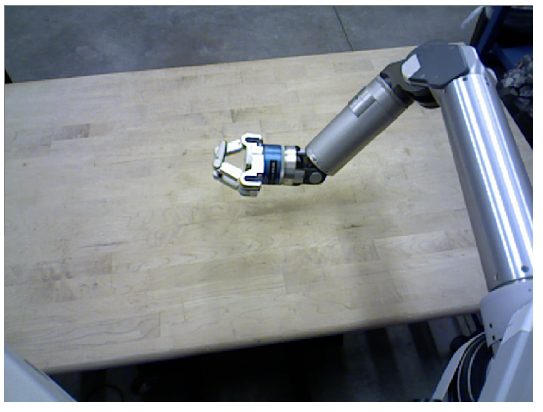
\includegraphics[width=1.0\textwidth]{img/dense_tracking/rgb_input}
		\caption{RGB input (not used)}
	\end{subfigure}
	\begin{subfigure}{0.45\textwidth}
		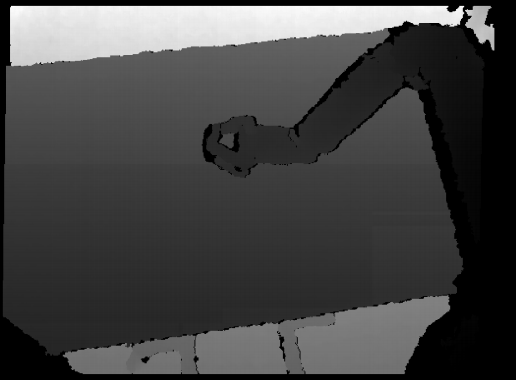
\includegraphics[width=1.0\textwidth]{img/dense_tracking/depth_input}
		\caption{Depth input}
	\end{subfigure}
	\begin{subfigure}{0.45\textwidth}
		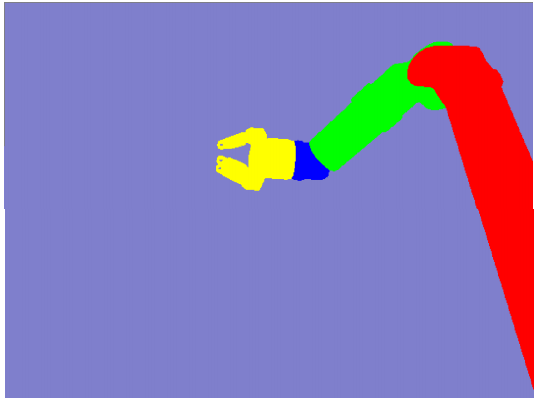
\includegraphics[width=1.0\textwidth]{img/dense_tracking/label_render}
		\caption{Synthetic label image}
	\end{subfigure}
	\begin{subfigure}{0.45\textwidth}
		\centering
		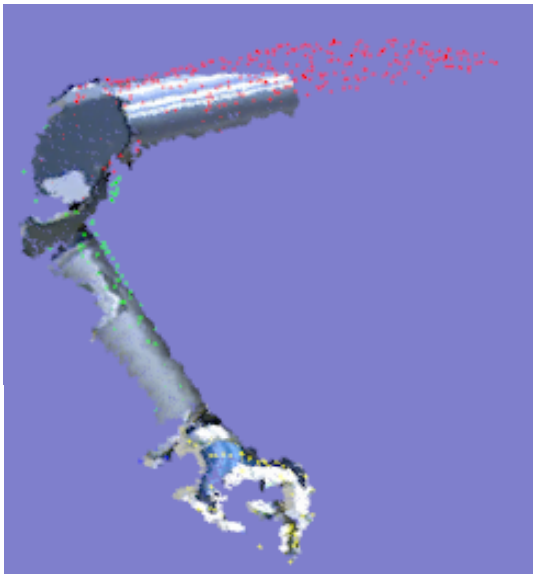
\includegraphics[width=0.75\textwidth]{img/dense_tracking/pointclouds}
		\caption{Synthetic and real point clouds}
	\end{subfigure}
	\caption{Images taken during different phases of the dense tracking algorithm.}
    \label{fig:dense_tracking}
\end{figure}

\subsection{Matching to the depth image}
Our implementation relies on quickly rendering and matching points of the robot's body to points in the point cloud. To achieve this, we render a \textit{synthetic point cloud} (\figref{fig:dense_tracking}) using a CAD model of the robot and the depth camera's intrinsics. Points are labeled by the GPU according to the link they are associated with. Each synthetic point is then matched to a real point in the point cloud using an octree. Outliers are rejected. The result is a conservative matching between the synthetic point cloud and the real one which naturally handles occlusion and segmentation.

\subsection{Stochastic gradient descent}
We compute the stochastic gradient of the log-likelihood function with respect to the robot's configuration by randomly sampling $M$ points of the robot's body and computing:

\begin{align}
	\frac{\partial}{\partial \config} \log \Prob(\DepthImage | \config) &\approx \sum_{i = 1}^{M}  \frac{\partial}{\partial \config}  \Prob(\pixel_i | \config) \\
		&= -\frac{1}{\sigma_\pixel}\sum_{i = 1}^{M} \J_{\beta_i}\trans\left(\pixel - \beta_i(\config)\right)
\end{align}

\noindent where $\J_{\beta_i}$ is the linear kinematic Jacobian of the robot arm evaluated for body point $\beta_i$ (\sref{sec:kinematics}). The gradient of the joint encoder posterior can also be computed as

\begin{align}
	\frac{\partial}{\partial \config} \log \Prob(\config | \enc) = -\frac{K_\enc(\enc_T) - \config}{\sigma_\config}
\end{align}

We use the stochastic gradient, rather than the full gradient, to save on computation. The gradient descent step is then:

\begin{equation}
	\config^{(k +1)} = \config^{(k)} - \lambda\left(\frac{\partial}{\partial \config} \log \Prob(\config | \enc) + \frac{\partial}{\partial \config} \log \Prob(\DepthImage | \config)\right)
\end{equation}

\noindent where $\lambda$ is a learning rate. We repeat until $\config^{(k)}$ converges, and becomes the new estimated state of the robot's joint angles.

\section{Experiments}

We tested the dense tracking algorithm on the DARPA ARM-S robot, which has an Asus \textit{Xtion Pro} depth sensor and a Barret WAM arm. Timing data for the tracker is shown in \tableref{tab:dense_track_time}. On average, the tracker runs at more than $100$ Hz (the majority of time being spent creating the synthetic point cloud image and shuffling data back and forth between the GPU). This is fast enough to incorporate into a real-time control loop for visual servoing.

\begin{table}
\centering
\begin{tabular} {l|l}
    Algorithm Step     & Average time per frame (ms) \\
    \hline
	Forward Kinematics & 0.1 \\
	Gradient Calculation & 0.2  \\
	Data Association & 1.5  \\
	Synthetic Rendering & 8.0
\end{tabular}
\caption{Timing data for the dense tracking algorithm. Notice that rendering the synthetic point cloud takes up the vast majority of the time. Altogether, the algorithm runs at $\sim100$ Hz.}
\label{tab:dense_track_time}
\end{table}

To verify that the algorithm was really reducing error in the robot's joint angles, we conducted an experiment where the robot was asked to touch a 2cm radius red dot repeatedly from different directions with randomly sampled inverse kinematics solutions. The red dot was detected using HSV blob segmentation in the RGB-D image, and its centroid in the point cloud was treated as the 3D target that the robot was to servo toward (\figref{fig:touching_track}). We measured how far the finger tip fell from the center of the red dot as a measure of accuracy. The experiment was performed 15 times for each case (with and without dense tracking), using the same randomly sampled starting end ending configurations for the arm.

\begin{figure}[width=1.0\textwidth]
\centering
\begin{subfigure}{0.4\textwidth}
	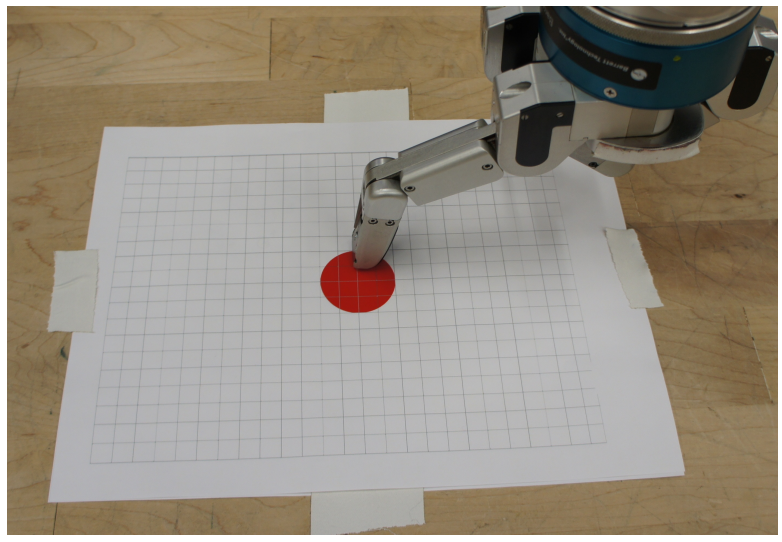
\includegraphics[width=1.0\textwidth]{img/dense_tracking/track_touch}
	\caption{}
\end{subfigure}
\begin{subfigure}{0.4\textwidth}
	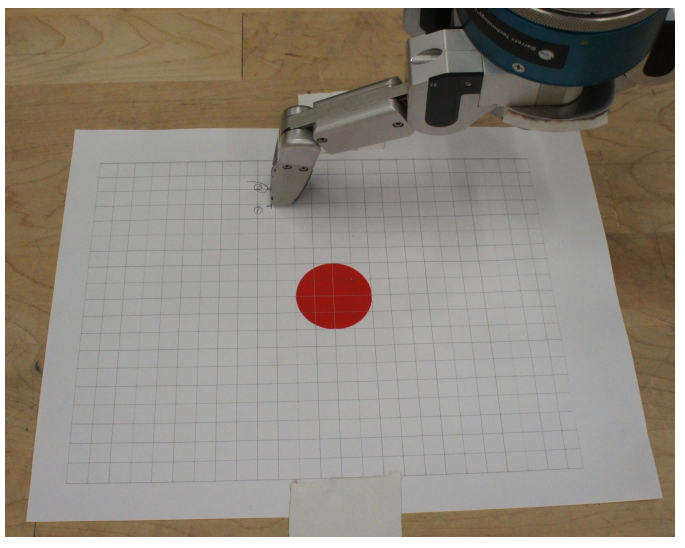
\includegraphics[width=0.9\textwidth]{img/dense_tracking/openloop_touch}
	\caption{}
\end{subfigure}
	\begin{subfigure}{0.5\textwidth}
	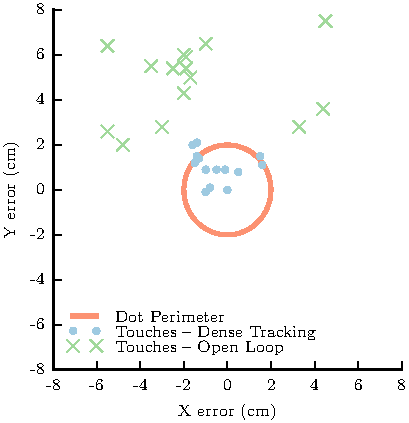
\includegraphics[width=0.9\textwidth]{img/dense_tracking/dots}
	\caption{}
	\label{fig:touching_data}
	\end{subfigure} 
\caption{The visual servoing experiment. Left: the robot servos toward the red dot while tracking its joint angles with the depth image. Right: the robot servos toward the red dot without tracking its joint angles with the depth image.}
\label{fig:touching_track}
\end{figure}

\figref{fig:touching_data} shows the error of the fingertip when using visual servoing and without. Tracking the arm in the depth image resulted in error that was well under 2cm, while using open-loop position control resulted in errors that were in excess of 7cm. 

This kind of error reduction allows us to perform more precise manipulation tasks. Figure \figref{fig:door_open} shows an example of such a task: the robot uses dense tracking to servo toward a door handle and open it. We performed this experiment 10 times. The robot was said to succeed whenever its fingers caged the door handle, and was said to fail whenever its fingers missed the door handle completely, collided with the door, or hit the door handle and slipped off. With visual servoing from dense arm tracking, the robot succeeded 9/10 times. With open-loop position control, the robot succeeded 0/10 times.

\section{Discussion and Limitations}
We have shown an example of how visual data can be used to correct joint angle uncertainty for a robot arm, and how this correction can be used to improve the robot's performance. The key idea behind this simple algorithm involves treating the problem as one of maximum likelihood estimation in the configuration space of the robot, given the sensor data.

However, this algorithm has severe limitations. First, it assumes all of the error comes from joint angle offsets along the axis of the robot's joints. It treats this uncertainty as simple isometric Gaussian noise on the joint encoders, when in reality the noise is likely to be nonlinear and depends on factors such as gravity and torque. 

The technique fails to explicitly estimate the uncertainty of the robot arm's state. Rather, it just estimates a single maximum-likelihood estimate. Because it makes the Markov assumption, the dense tracker does not make use of the entire robot trajectory to estimate the state. This makes the technique prone to local minima.

Because we use simple point-to-point data associations between the robot's body and the depth image, we run the risk of mismatching data. Because we rely on simple gradient descent to optimize the log-likelihood function, the algorithm is not very robust to outliers caused by mis-matching of data. This will occur if any un-modeled objects (such as objects held in the robots hand, or surfaces occluding the arm) are visible in the depth image near the arm.

Finally, this technique relies on a depth camera that can see all or part of the robot's arm. What do we do if the camera is mounted on the robot's hand (and hence can't see any part of the robot's arm)? What if depth is not available? We will tackle some of these problems in the next two chapters.
\chapter{Dense Tracking and Mapping with a Hand-Mounted Depth Sensor} \label{chap:dense_slam}
\lettrine{C}onsider the following scenario: a robot with a hand-mounted depth sensor scans an unknown scene filled with clutter. The robot's goal is to create a geometric model of the scene that it can use for motion planning and manipulation. If the robot had perfect kinematics, and no uncertainty in its joint angle estimates, creating a geometric map of the scene would be trivial -- it would just involve finding the pose of the sensor at each timestep by looking at the robot's joint encoders, and then stitching together all of the robot's sensor measurements at each pose to create a 3D model. Unfortunately, as we have seen in the previous chapters, many robots do not have perfect joint angle sensing, and some robots have a very large amount of kinematic error. With incorrect joint angle measurments, the model of the scene that the robot creates from its scan will be inaccurate.

\begin{figure}[width=0.5\columnwidth, ht]
	\centering
	\begin{subfigure}{0.5\columnwidth} 
	\centering
	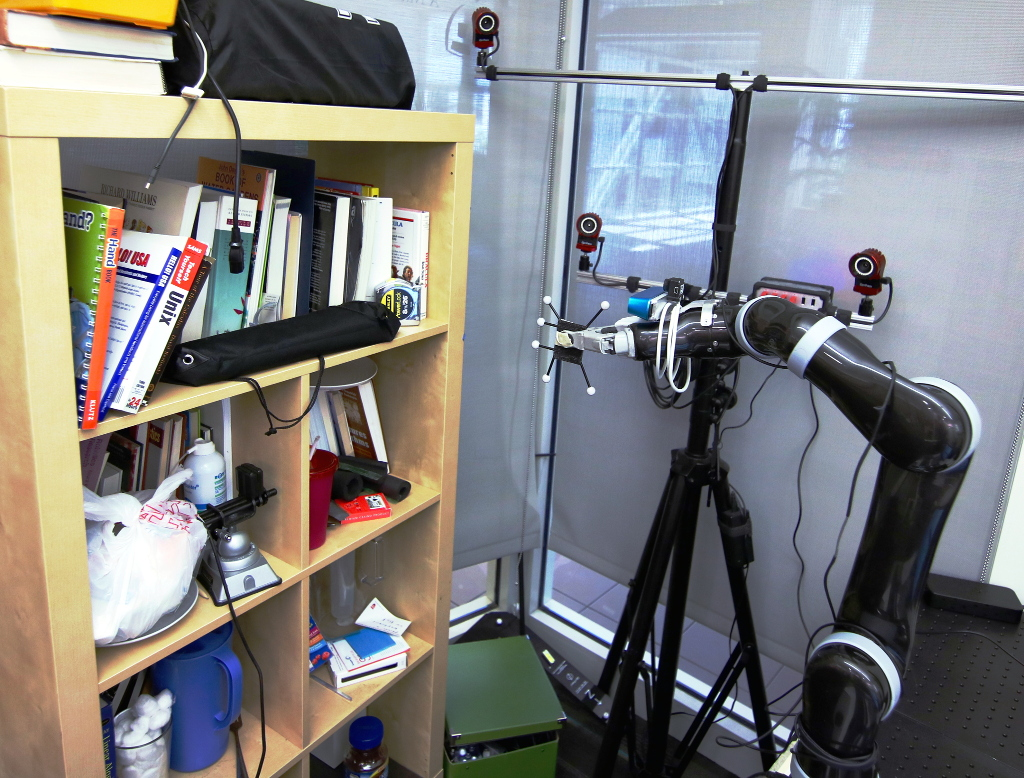
\includegraphics[width=1.0\textwidth]{img/arm_slam/experimental_setup.JPG}
	\caption{Experimental setup.}
	\label{fig:real_robot}
	\end{subfigure}
	 \begin{subfigure}{0.29\columnwidth}
	 \centering 
	 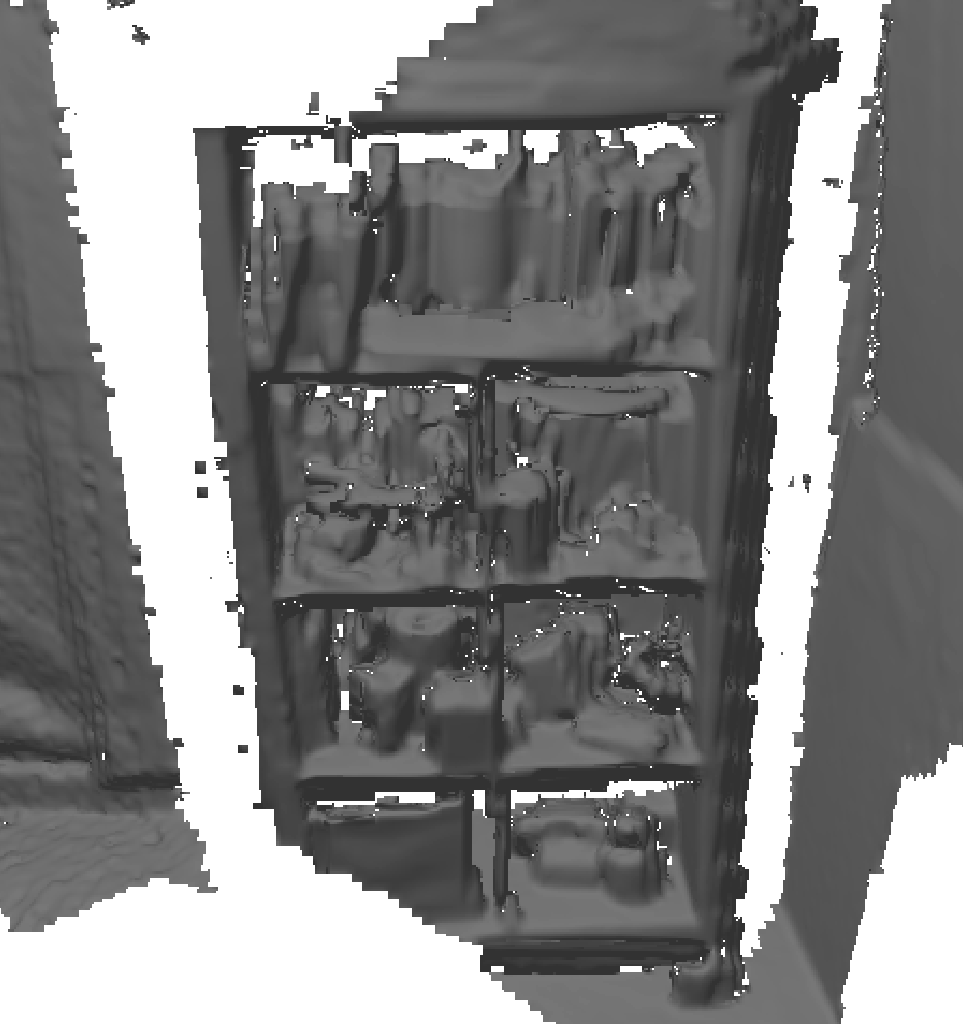
\includegraphics[width=1.0\textwidth]{img/arm_slam/kinfu_bookshelf.png}
	 \caption{Kinect Fusion (baseline).}
	 \end{subfigure}
	\begin{subfigure}{0.29\columnwidth}
	\centering
	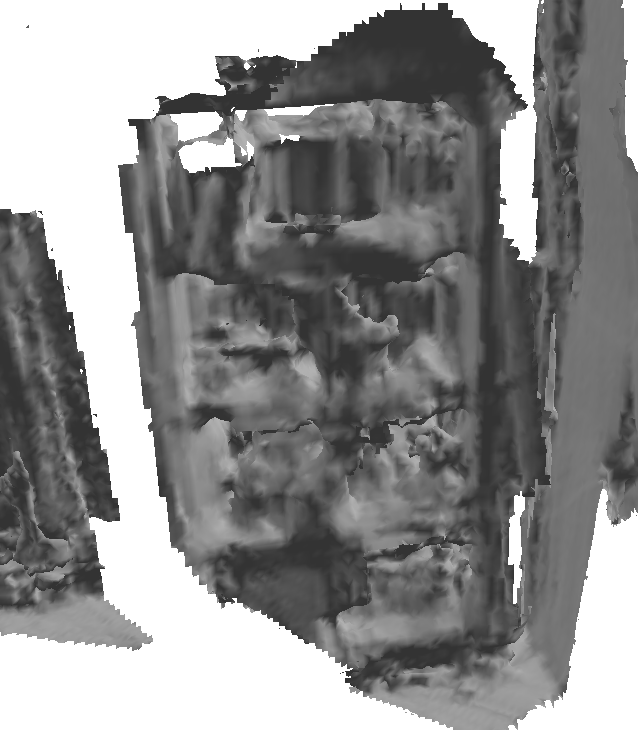
\includegraphics[width=1.0\textwidth]{img/arm_slam/lambert_bookshelf_notrack.png}
	\caption{Forward kinematics. }
	\end{subfigure}
	\begin{subfigure}{0.29\columnwidth}
	\centering 
	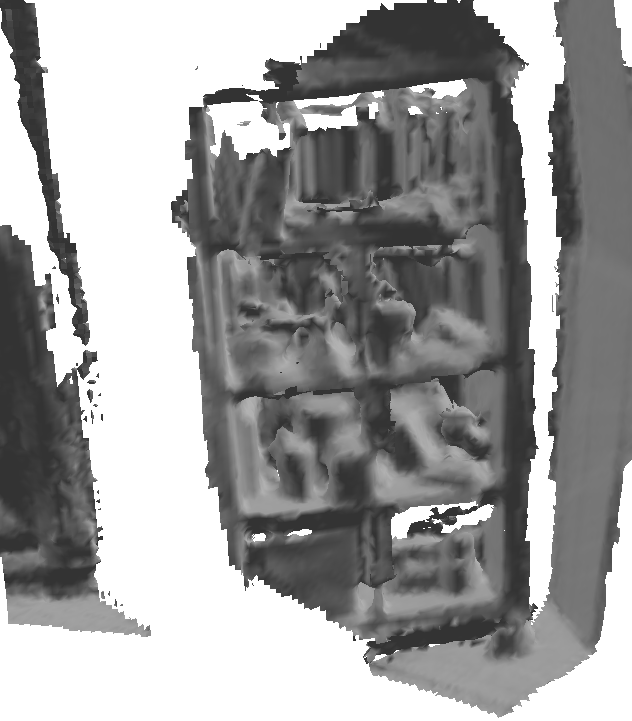
\includegraphics[width=1.0\textwidth]{img/arm_slam/lambert_bookshelf.png}
	\caption{ARM-SLAM}
	\end{subfigure}
	  \begin{subfigure}{0.29\columnwidth}
	 \centering
	 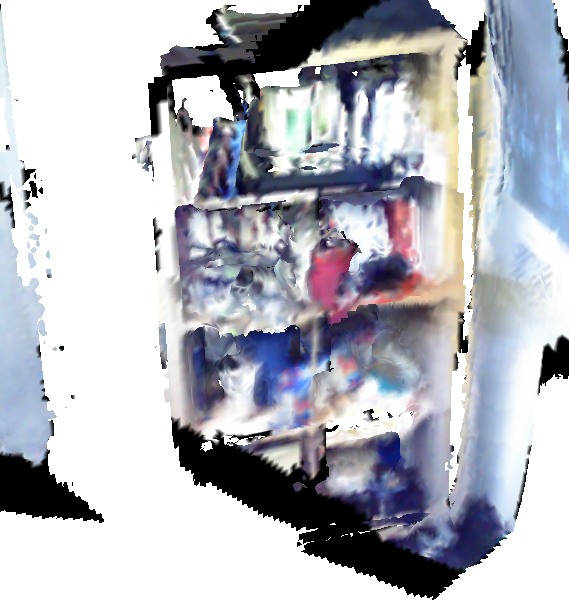
\includegraphics[width=1.0\textwidth]{img/arm_slam/better_bookshelf.png}
	 \caption{Colorized ARM-SLAM.}
	 \end{subfigure} 
	\caption{Robot scans and reconstructions of a bookshelf at 1.5cm resolution using real depth and encoder data (\sref{sec:3d_real}). Our approach (which estimates robot configurations rather than camera poses) results in preservation of fine detail and edges that are lost when only using the robot's forward kinematics, with comparable reconstruction quality to Kinect Fusion.}
	\label{fig:real_reconstructions}
\end{figure}

As we have seen in chapter \ref{chap:dense_external_tracking}, an external depth sensor mounted on a robot's body or affixed somewhere in the scene can be used to correct joint angle error by maximizing the likelihood of a robot's configuration given its sensor data.Can the same approach that we discussed in \ref{chap:dense_external_tracking} be used when the camera is mounted on the robot's hand, and can't see any part of the robot's body? 

Right away, it's clear that we're dealing with a Simultaneous Localization and Mapping (SLAM) problem. The robot's pose at any given time is unknown because of kinematic uncertainty. The model of the world is likewise unknown \apriori. We will therefore have to estimate both the structure of the world and the robot's state simultaneously.

In this chapter, we will explore a dense SLAM technique which simultaneously estimates the robot's joint angles and a dense 3D geometric model of the world \footnote{This chapter is largely restating earlier work found in \cite{Klingensmith2016}}.

\section{Problem Definition}
We have a series of discrete time steps $t = 1, \ldots T$ with synchronized joint encoder measurements $\enc_1, \ldots, \enc_T$ and depth images $\DepthImage_1, \ldots, \DepthImage_T$. The task is to estimate the robot's true configuration $\config_1, \ldots \config_T$ and a geometric model of the scene $\DenseMap$ simultaneously. Formally, we can express this as computing a maximum likelihood estimate of the robot's trajectory and geometric model

\begin{equation}
	\left\{\config_1, \ldots, \config_T, \DenseMap\right\}_{\text{MLE}} = \argmax_{\config_1, \ldots, \config_T, \DenseMap} \Prob\left(\config_1, \ldots, \config_T, \DenseMap | \DepthImage_1, \ldots, \DepthImage_T, \enc_1, \ldots, \enc_T\right)
\end{equation}

\noindent this expression is extaordinarily high-dimensional, and is difficult to directly optimize it, because the dense model $\DenseMap$ correlates every sensor measurement together. Therefore, we solve this problem in the same way as several other dense SLAM techniques (particularly \textit{Kinect Fusion}~\cite{KinectFusion}) by breaking the problem into two parts: first, tracking the sensor with respect to a fixed dense map, and second, updating the dense map with respect to a fixed sensor pose.These two steps, performed rapidly in alteration can be made to simultaneously construct a map and track the pose of the sensor. The trade off is that both the pose and structure of the map can drift over time as small errors accumulate.

\subsection{Mapping the Scene}
Given a set of depth images $\DepthImage_1, \ldots, \DepthImage_T$ taken at known poses $C_1, \ldots, C_T$, we wish to construct a 3D geometric model of the scene $\DenseMap$. This is a well-studied problem in computer vision. We chose the volumetric method of Curless and Levoy \cite{Curless1996} known as Truncated Signed Distance Field (TSDF) mapping. This is the same mapping method used by \textit{Kinect Fusion} \cite{KinectFusion}.

Using this method, the 3D model takes the form of a volumetric signed distance function:

\begin{equation}
	\DenseMap = \Phi(\xvec) : \RThree \to [-\tau, \tau]
\end{equation}

\noindent where $\tau$ is a small radius around the surfaces of objects. The  TSDF maps volumetric points in the scene $\xvec$ to their distance to the nearest surface. Inside objects, the the distance is negative, and outside the distance is positive. Exactly at the surface, the distance is zero. Therefore, the surface of the scene is implicitly represented as the level set $\Phi(\xvec) = 0$.

To generate a TSDF from a series of depth images, we take all the points $\pixel_i \in \DepthImage$ in the point cloud of each depth image, compute its surface normal $\mathbf{n}_i$, and use this to construct a linearization of the distance field near $\pixel_i$. For all of the points $\xvec$ within a radius $\tau$ of $\pixel_i$, we set its signed distance $\Phi(\xvec)$ to the linearized value derived from the surface normal. When the linearizations of several pixels intersect, we merely average the distances. Curless \cite{Curless1996} proved that this method minimizes the squared distance of points in the point cloud to the implicit surface generated by $\Phi$.

In practice, this is accomplished by storing voxels $V$ within a region of interest. Each discrete voxel contains an estimate of the signed distance, and a weight which is used to produce a running average of the TSDF as new measurements accumulate. Algorithm \ref{alg:TSDF} describes how to fuse a new depth image at a known pose into the TSDF.

\begin{algorithm}
\tcp{Given a depth image, sensor pose, previous TSDF, previous voxel weights, a weighting function, a volume of interest, and a truncation distance}
\KwIn{$\DepthImage, C, \Phi^{(t - 1)}, W^{(t - 1)}, w,  V, \tau$}

\tcp{Inverse of the camera transform}
$C' \gets {C}^{-1}$

\tcp{Initialize the new TSDF to the previous one}
$\Phi_{t} \gets \Phi_{t - 1}$

\tcp{Initialize the weights}
$W_{t} \gets W_{t - 1}$

\For{$\mathbf{v} \in V$}
{
    \tcp{Depth of voxel $\mathbf{v}$}
    $\mathbf{v}_c \gets C' \mathbf{v}$
	
	\tcp{Current depth measurement for the voxel.}
	$d_i \gets \DepthImage\left[\Proj(\mathbf{v}_c)\right]$
	
	\tcp{Dist to camera plane.}
	$d_v \gets \mathbf{v}_{c}(z)$
	
	\tcp{Locally linear approximation.}
	$u \gets d_v - d_i$
	
	\tcp{If dist within $\tau$}
	\If{$|u| < \tau$}
	{
	    \tcp{Weighted average}
		$\Phi_{t}(\mathbf{v}) \gets \frac{W_{t}(\mathbf{v}) \Phi_{t}(\mathbf{v}) + w(u) u}{W_{t}(\mathbf{v}) + w(u)}$
		
		$W_{t}(\mathbf{v}) \gets W_t(\mathbf{v}) + w(u)$
	}
}
 
\KwOut{$\Phi_{t}, W_{t}$}
\caption{\textsc{FuseTSDF}}
\label{alg:TSDF}
\end{algorithm}

Using a TSDF to model the scene allows us to average out sensor measurement error as depth images accumulate. The TSDF, since it is continuous and volumetric, also has the advantage of having well-defined gradients $\nabla \Phi$, which are easy to compute using finite differencing.

\subsection{Tracking the Arm}
Assuming a fixed dense map $\DenseMap$, the problem of tracking the arm becomes significantly easier, since we can use the Markov assumption such that the current configuration of the robot is conditionally independent of all the previous configurations, joint encoder measurements and depth images:

\begin{align}
	\config_{\text{MLE}} &= \argmax_{\config} \Prob\left(\config | \DepthImage_T, \enc_T, \DenseMap\right) \\
						 &= \argmax_{\config} \frac{\Prob\left(\DepthImage_T | \config, \DenseMap\right)\Prob\left(\config | \enc_T\right)}{\Prob(\DepthImage_T, \enc_T, \DenseMap)} \\
						 &= \argmax_{\config} \log \Prob(\DepthImage_T | \config, \DenseMap) + \log \Prob(\config | \enc_T)				 
						 \label{eqn:dense_map_track}
\end{align}

\noindent notice that \eqnref{eqn:dense_map_track} bears a striking resemblance to \eqnref{eqn:dense_model_track}, only with an additional term for the dense map $\DenseMap$. This is because with a known map, the problem of tracking the robot arm using a depth image of its own body is exactly equivalent to tracking the robot arm using a depth image of a rigid body attached to its base. In this context, the dense map of the scene can be seen as \textit{just another link} of the robot that is attached rigidly to its base.

With this framework in mind, it is possible to use the same algorithm as in chapter \ref{chap:dense_external_tracking} to track the robot, replacing points on the robot's body with points in the dense map. This is essentially what we do in \cite{Klingensmith2016}, except our representation of the dense map $\DenseMap$ is volumetric, rather than point-based. The joint encoder posterior here is exactly the same as in \eqnref{eqn:dense_model_track}, so we use the same method to compute it.

\subsubsection{Depth Image Posterior}
Assume that the points in the depth image are really samples of points on the surface of $\DenseMap$ that have been corrupted by isotropic Gaussian noise. That is, for each $\pixel_i \in \DepthImage$, assume that there exists a point $\xvec_i~\text{s.t}~ \Phi(\xvec_i) = 0$ that corresponds to a point on the surface of $\DenseMap$, and

\begin{equation}
	\pixel_i \sim \xvec_i + \mathcal{N}(0, \Sigma_\pixel)
\end{equation}

\noindent where $\Sigma_\pixel = \sigma_\pixel \eye$, and $\sigma_\pixel$ is the variance of the depth image noise. If $\pixel_i$ is already very close to $\xvec_i$, then the value of the distance field $|\Phi(\pixel_i)| \approx \|\pixel_i - \xvec_i\|$, and therefore

\begin{equation}
	\Prob\left(\pixel_i | \DenseMap\right) \approx \exp{\frac{-\|\Phi(\pixel_i)\|^2}{2 \sigma_\pixel}}
\end{equation}

Assuming conditional independence among all the pixels in the depth image, we arrive at the expression for the log-likelihood of the depth image posterior from equation \ref{eqn:dense_map_track} as

\begin{align}
	\log \Prob(\DepthImage | \config, \DenseMap) &\approx \log \prod_{\pixel_i \in \DepthImage} \exp{\frac{-\|\Phi(\pixel_i)\|^2}{2 \sigma_\pixel}} \\
				&= -\frac{1}{2 \sigma_\pixel}\sum_{\pixel_i \in \DepthImage}\Phi(\pixel_i)^2 
				\label{eqn:log_likelihood_dense_map}
\end{align}

\noindent note that this is only valid if the pose estimate is already very near the true pose of the sensor. Otherwise, the points from the depth image may be mis-matched to points in the dense map. Depending on the geometry of the scene, the mis-matching could be more or less severe. For instance, if the world consists of a single plane, this method would not be able to distinguish between points on the plane, and all poses that move parallel to the plane will be treated as equally probable (this is a problem that other TSDF methods suffer from as well).

\section{Algorithm Implementation}
As in chapter \ref{chap:dense_external_tracking}, we use stochastic gradient descent of the log-likelihood function to obtain a pose estimate for the robot arm. We interleave this pose estimation step with a TSDF mapping step following \algref{alg:TSDF}. The result is a system which generates a consistent 3D map and corrects the robot's joint angles in real time.

\subsection{TSDF Mapping}
We use the TSDF mapping system from our earlier work \cite{Klingensmith2015}. This mapping system (called \textsc{Chisel}) represents the TSDF as a spatial hash map of voxels. Each voxel stores a 16-bit signed distance, a 16-bit weight, and a 32-bit color (which is not used for tracking). The TSDF grows as more surfaces are observed, but unlike other systems, \textsc{Chisel} stores only voxels that are near surfaces, rather than the entire scene. This allows very large scale maps to be stored efficiently.

\subsection{Stochastic Gradient Descent}
The gradient of the log-likelihood function expressed in \eqnref{eqn:log_likelihood_dense_map} with respect to the robot's configuration $\config$ can be computed as a simple application of the chain rule

\begin{equation}
	\frac{\partial}{\partial \config} \log \Prob(\DepthImage | \config, \DenseMap) = -\frac{1}{2 \sigma_\pixel} \sum_{\pixel_i \in \DepthImage}\Phi(\pixel_i)\J_{\pixel_i}\trans \nabla \Phi(\pixel_i)
\end{equation}


\begin{algorithm}

\tcp{Where $\qvec_e^{(t)}$ are the motor encoders at time $t$,  $\lambda$ is a learning rate, and $\gamma$ is a regularization parameter.}
\KwIn{$\DepthImage_t, \enc_t, \Phi^{(t - 1)}, \lambda, \config^{(t- 1)}$}

$\config^{(k)} \gets \config^{(t - 1)}$

\Repeat{\text{convergence}}
{
	\tcp{The camera transform given the robot's joint angles.}
    $T_{\qvec} \gets F_{\text{cam}}(\qvec^{(k)})$
    
	\tcp{Gradient of the depth image posterior.}
	$\nabla C \gets  \frac{1}{\sigma_\pixel}\sum_{\pixel \in \DepthImage_t} \left[\Phi^{(t - 1)}\left[T_{\qvec} \pixel\right] \mathbf{J}_{\pixel}^T\nabla \Phi^{(t - 1)}\left[T_{\qvec} \pixel\right]\right]$
	
	\tcp{Descend the gradient.}
	$\config^{(k)} \gets \config^{(k)} - \lambda\left(\nabla C  + \frac{1}{\sigma_\config}\left(\qvec - K_\enc(\enc_t)\right)\right)$
}

$\config_t \gets \config^{(k)}$

\tcp{Mapping step.}
$\Phi^{(t)} \gets \textsc{FuseTSDF}\left(\Phi^{(t - 1)}, \DepthImage_t, \configc_t\right)$
 
\KwOut{$\config_t, \Phi^{(t)}$}
\caption{ARM-SLAM}
\label{alg:artfu}
\end{algorithm}

\section{Experiments}
\label{sec:experiments}
 
We conducted three types of experiments to observe the behavior of this algorithm; 2D simulation experiments, 3D simulation experiments, and a real robot experiment. \footnote{\textit{Videos are available at \texttt{http://youtu.be/QrFyaxFUs9w}}}

\subsection{2D Simulation}
\label{sec:2D_sim}
In the simple 2D simulation experiment, a 3-link serial robot manipulator with a simulated 1D depth sensor scans a scene. We added zero-centered Perlin \cite{Perlin02} noise to its joint encoder readings. That is,
 %
\begin{equation}
\enc_t = \config_t + \beta_n\textsc{Perlin}\big(s_n \config_t\big)
\end{equation}

\noindent where $s_n, \beta_n$ are parameters which control noise frequency and magnitude, respectively. In our experiments, $s_n=1.0, \beta_n=0.2$. The simulated depth image is noiseless.

For the world model, we constructed a  simple 2D {TSDF}. We compare the performance of ARM-SLAM (\algref{alg:artfu}) against a simple unconstrained descent algorithm which assumes the sensor can move and rotate freely, without considering the robot kinematics (\figref{fig:2d_experiment}). We found that ARM-SLAM managed to both reduce end effector error and dramatically reduce model error (\tableref{table:2d_experiment_data}), whereas just using a 2D dense fusion technique without constraining using the robot's kinematics resulted in severe, unrecoverable drift because of the scene's self-similarity and the robot's fast motion. Note that in the real experiments, there is comparatively much less actuator noise, and a much smaller scene than in the 2D experiments.

\begin{figure}[ht]
\centering
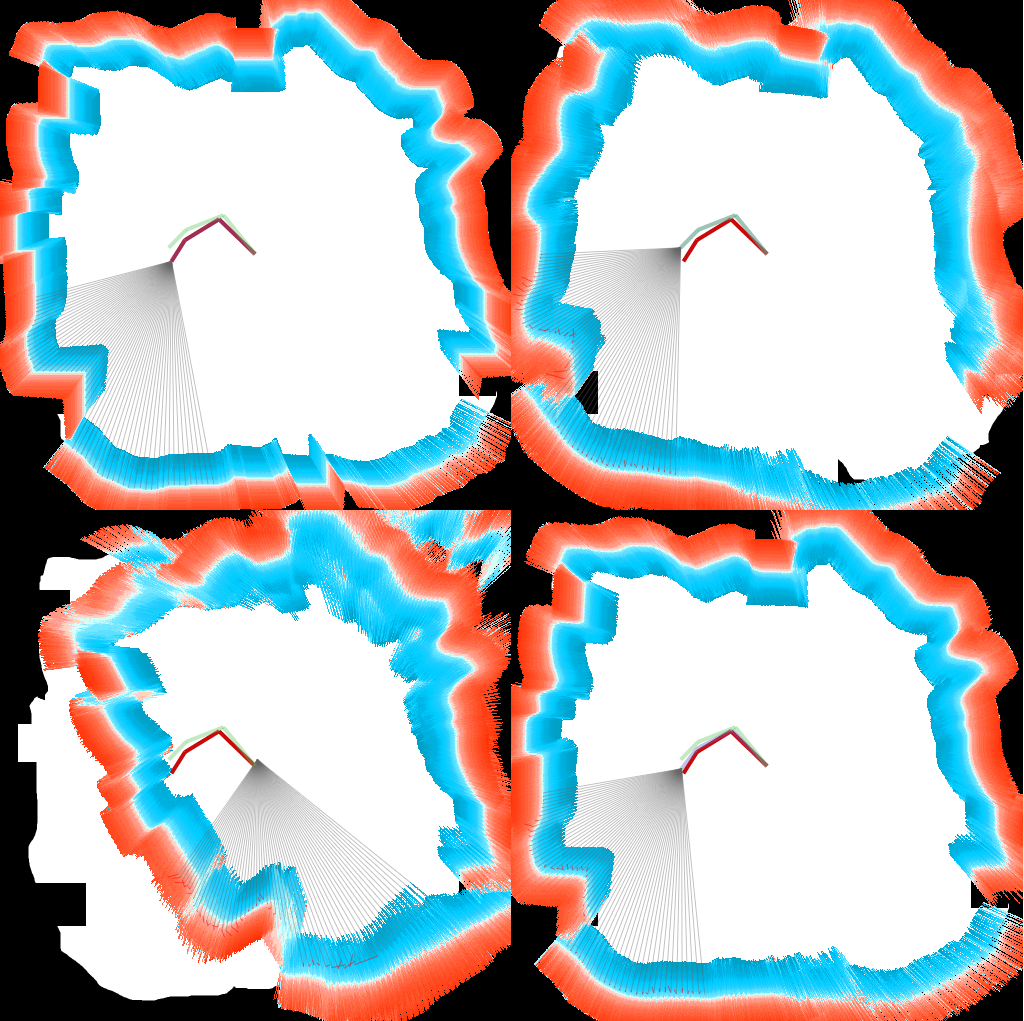
\includegraphics[width=0.78\columnwidth]{img/arm_slam/2d_experiments/2d_end.png}
\caption{2D simulation experiment (\sref{sec:2D_sim}). The robot is shown in red. The simulated depth image is shown as grey rays. The TSDf is shown as orange or blue pixels. Top left shows the ground truth {TSDF}, top right is with forward kinematics only (with actuator uncertainty). Bottom left corrects actuator noise using unconstrained dense fusion. Bottom right corrects using ARM-SLAM.}
\label{fig:2d_experiment}
\end{figure}

\begin{table}
 \begin{tabular}{*5l}
          \hline
             $t$ &      & \textit{Fwd. Kin.}  & \textit{Dense Fusion} & \textit{ARM-SLAM} \\ \hline
             \multirow{4}{*}{500} & EE Err. (pix.)      & $5.2 \pm 5.9$ & $3.4 \pm 4.2$ & $\mathbf{0.8 \pm 0.7}$ \\ 
              & Jnt. Err (rad.)                 & $0.08 \pm 0.06$ & $ - $ & $\mathbf{0.06 \pm 0.05}$ \\
              & SDF Err (pix.)                  & $1.4 \pm 1.7$ & $0.8 \pm 0.8$ & $\mathbf{0.5 \pm 0.3}$ \\ 
              & Class Err (\%)                     & $5.7 \pm 3.2$ & $4.7 \pm 2.3$ & $\mathbf{3.5 \pm 0.6}$ \\ \hline
              
              \multirow{4}{*}{999} & EE Err. (pix.)    & $9.2 \pm 6.7$ & $14.7 \pm 17.8$ & $\mathbf{1.4 \pm 1.9}$ \\ 
              & Jnt. Err (rad.)                   & $0.17 \pm 0.07$ & $ - $ & $\mathbf{0.08 \pm 0.05}$ \\
              & SDF Err. (pix.)                   & $6.1 \pm 5.3$ & $12.2 \pm 22.2$ & $\mathbf{1.2 \pm 0.8}$ \\ 
              & Class Err. (\%)                     & $11.3 \pm 6.2$ & $9.5 \pm 6.1$ & $\mathbf{4.4 \pm 1.1}$ \\
              \hline
    \end{tabular} 
    \caption{Results for the 2D simulation experiments (\sref{sec:2D_sim}). The end effector error in pixels, joint angle error in radians, distance field error in $10^6$ pixels, and occupancy classification error (the proportion of pixels misclassified as containing an obstacle) is shown for forward kinematics, unconstrained dense fusion, and ARM-SLAM for a dataset with 500 and 999 time-steps. Our approach (ARM-SLAM) reduces all three error terms.}
    \label{table:2d_experiment_data}
\end{table}

%\begin{figure}
%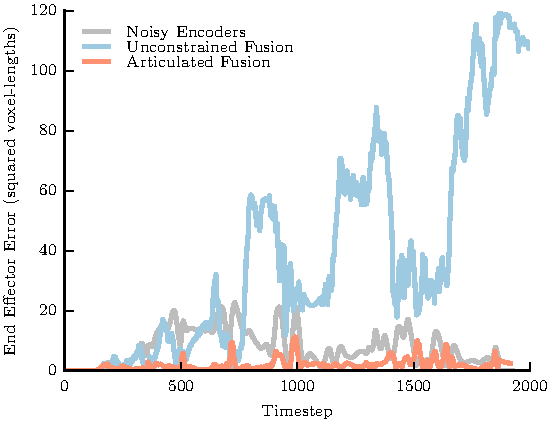
\includegraphics[width=1.0\columnwidth]{img/2d_experiments/ee_error.pdf}
%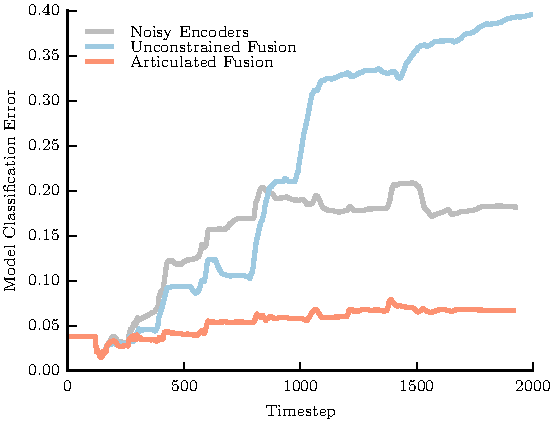
\includegraphics[width=1.0\columnwidth]{img/2d_experiments/class_error.pdf}
%\caption{2D experiment (\sref{sec:2D_sim}) data. Here, end effector error is the squared distance between the reported end %effector position and ground truth. The model classification error is the proportion of \ac{TSDF} voxels that are misclassified (full vs. empty).}
%\label{fig:2d_experiment_data}
%\end{figure}

\subsection{3D Simulation}
\label{sec:3d_sim}

We developed a 3D simulation of a Kinova \textit{Mico} robot with a hand-mounted Occipital \textit{Structure} \cite{StructureSensor} depth sensor. In the simulation, the robot scans a simulated bookshelf. As in the 2D experiments, Perlin noise is added to the ground truth joint angles to simulate actuator uncertainty. We use the \textit{Open Chisel} \cite{Klingensmith2015} chunked {TSDF} library for mapping. The simulated depth image is noiseless. Reconstructions were done at a resolution of 1.5 cm per voxel.

We found that ARM-SLAM was able to correct for very large actuator error (see \figref{fig:3d_experiment_data}), resulting in a final reconstruction near the ground truth (\figref{fig:3d_experiments}). By artificially increasing the actuator noise, we found that ARM-SLAM significantly reduced the end effector error even when the uncertainty in the camera's pose was up to 12 cm (\figref{fig:3d_exp_added_noise}), we also found ARM-SLAM to be more robust to tracking failure from lost data than unconstrained Kinect Fusion (\figref{fig:3d_exp_kinfu}) due to the very strong motion prior from the robot kinematics.

\begin{figure}[ht!]
\centering
\begin{subfigure}{0.4\columnwidth}
	\centering
	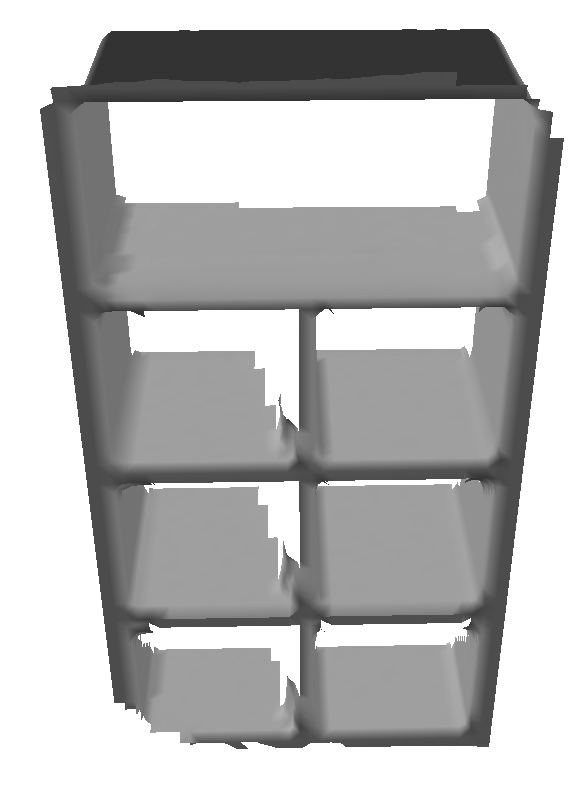
\includegraphics[height=1.0\textwidth]{img/arm_slam/groundtruth_sim.png}
	\caption{Ground truth}
\end{subfigure}
\begin{subfigure}{0.4\columnwidth}
	\centering
	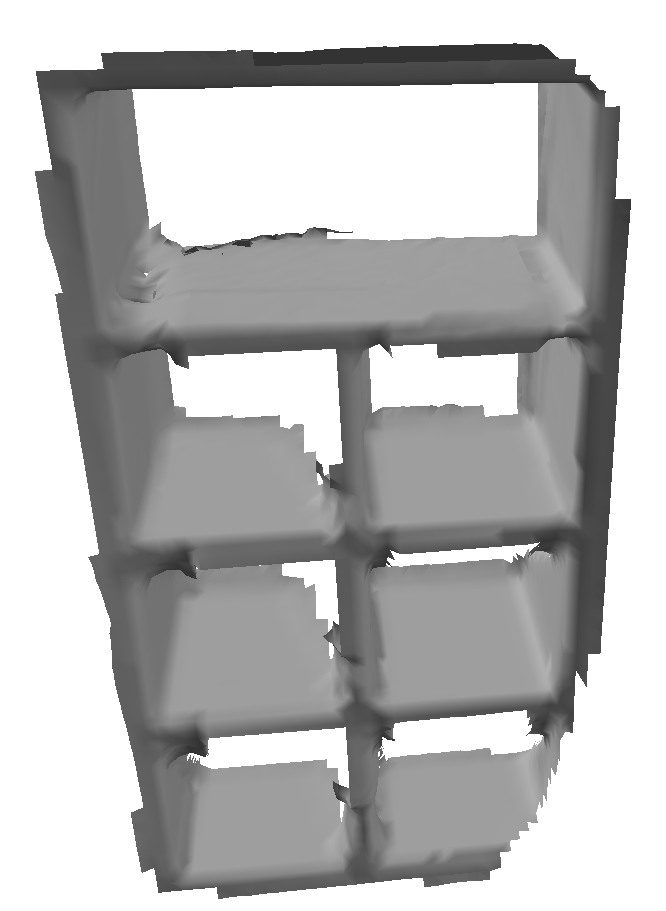
\includegraphics[height=1.0\textwidth]{img/arm_slam/artfu_sim.png}
	\caption{ARM-SLAM}
\end{subfigure}
\begin{subfigure}{0.4\columnwidth}
	\centering
	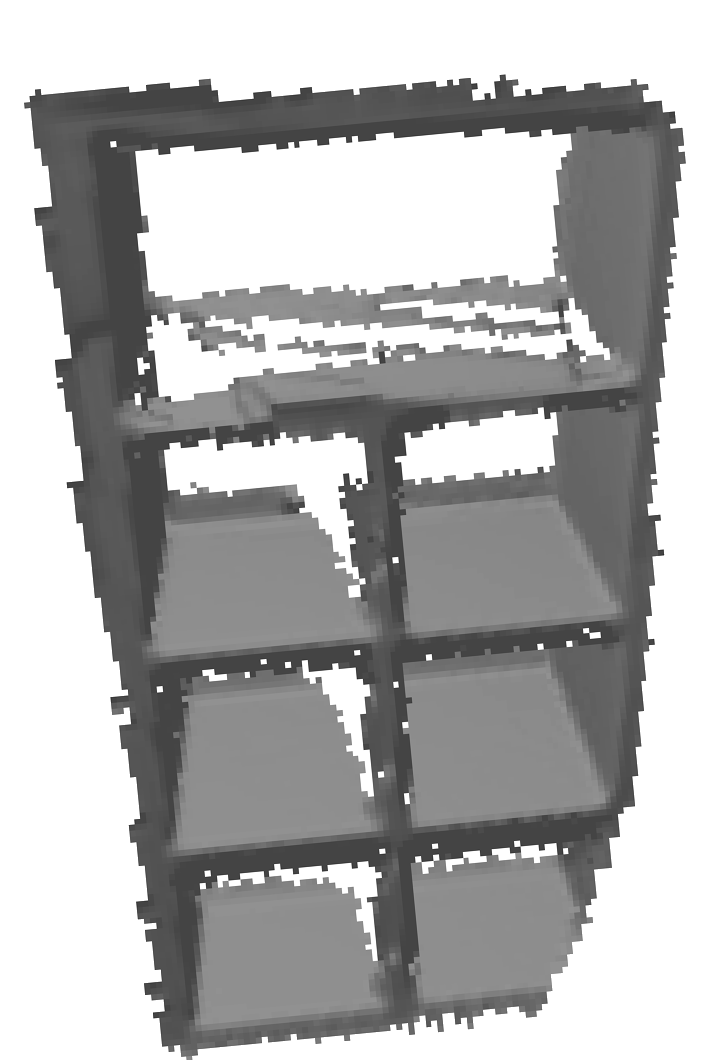
\includegraphics[height=1.0\textwidth]{img/arm_slam/kinfu_sim.png}
	\caption{Kinect Fusion}
\end{subfigure}
\begin{subfigure}{0.4\columnwidth}
	\centering
	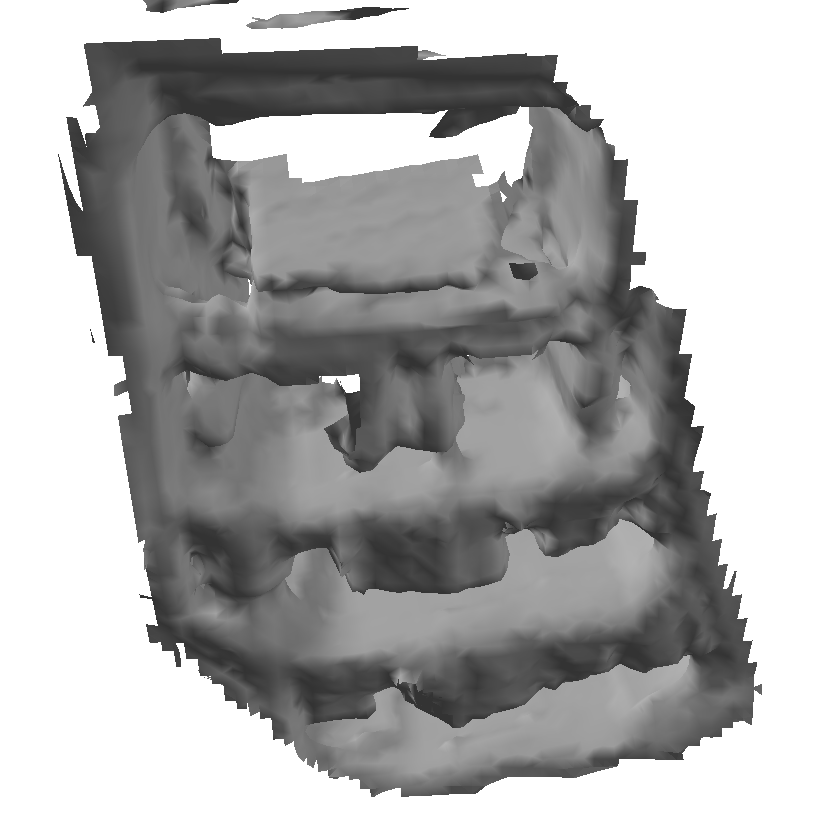
\includegraphics[height=1.0\textwidth]{img/arm_slam/kinematics_sim.png}
	\caption{Forward kinematics}
\end{subfigure}
\caption{Results of the 3D simulation (\sref{sec:3d_sim}) with up to 0.8 radians of added noise per joint.}
\label{fig:3d_experiments}
\end{figure}

\begin{figure}[ht]
\begin{subfigure}{0.5\columnwidth}
	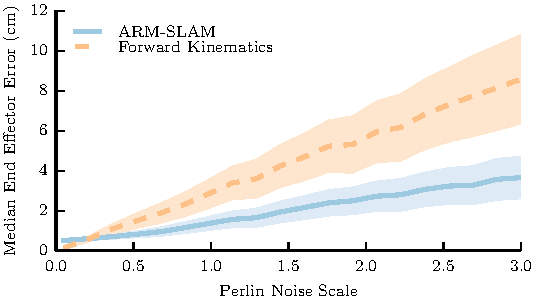
\includegraphics[width=1.0\columnwidth]{img/arm_slam/added_noise.pdf} 
	\caption{3D simulation with added noise.}
	\label{fig:3d_exp_added_noise}
\end{subfigure}
\begin{subfigure}{0.5\columnwidth}
	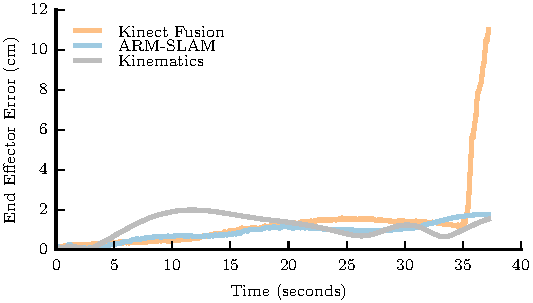
\includegraphics[width=1.0\columnwidth]{img/arm_slam/3d_kinfu_error.pdf} 
	\caption{3D simulation with lost tracking.}
	\label{fig:3d_exp_kinfu}
\end{subfigure} 
\begin{subfigure}{0.5\columnwidth}
	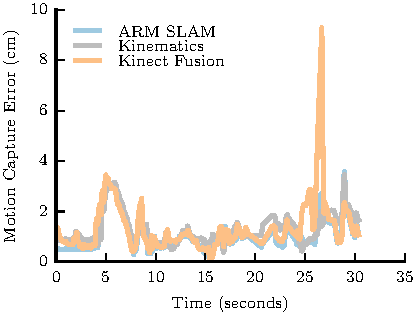
\includegraphics[width=1.0\columnwidth]{img/arm_slam/motion_track.pdf} 
	\caption{Real data validated with motion capture.}
	\label{fig:motion_track} 
\end{subfigure} 
\caption{End effector error observed in the 3D simulation (\sref{sec:3d_sim}) experiments. \figref{fig:3d_exp_added_noise}: 100 trials with different noise seeds are run with increasing noise magnitude. Each trial lasts 60 seconds. The median deviation of the end effector from ground truth is recorded. \figref{fig:3d_exp_kinfu}: in a different simulation, the robot briefly looks away from the scene and then looks back. Kinect Fusion loses tracking. \figref{fig:motion_track}: end-effector deviation in the real dataset as measured by an optical motion capture system, Kinect Fusion briefly loses and then regains tracking.}
\label{fig:3d_experiment_data} 
\end{figure}

\subsection{Bookshelf Scanning}
\label{sec:3d_real}

Using the same framework as in the 3D simulation, we reconstructed a bookshelf with a Kinova \textit{Mico} robot with a hand-mounted Occipital \textit{Structure} sensor (\figref{fig:real_reconstructions}). The robot was teleoperated using a joystick. Beforehand, the Structure sensor was extrinsically calibrated to the robot's hand using the Tsai\cite{Gupta11cameracalibration} method and a fiducial, though extrinsic calibration error cannot be ruled out. The end effector deviation was measured using an \textit{Optitrack} motion tracking system. One challenge of working with the real robot data is that the joint encoders and depth sensor are not synchronized. The joint encoder data is emitted at $\sim 500~\text{Hz}$, whereas the camera data is produced at $30~\text{Hz}$. To compensate for this, we store the robot's configuration space trajectory as a series of linearly interpolated, timestamped waypoints. Using this, we can infer the joint encoder readings at the time when the depth image was received. 

The 3D reconstructions (\figref{fig:real_reconstructions}) show that our method is able to recover 3D structure in the scene that is lost when only the (noisy) forward kinematics are used. This is especially apparent around the edges of the bookshelf and its adjacent walls. Our reconstructions are comparable to Kinect Fusion run at the same voxel resolution (1.5 cm). We measured end-effector motion with an optical 
motion capture system (\figref{fig:motion_track}) and found that Kinect fusion occasionally lost (and regained) tracking due to self-similar surfaces in the bookshelf and surrounding walls. Because of the strong motion prior from the robot's joints ARM-SLAM did not have this issue. However, our data from the motion capture system is too noisy to conclude ARM-SLAM performed any better than forward kinematics at reporting the true pose of the end effector (ARM-SLAM had an end effector deviation of $1.2 \pm 0.9 \text{cm}$ while forward kinematics had a deviation of $1.4 \pm 1.0 \text{cm}$). It may be that extrinsic calibration error between the sensor and rigid hand mount is dominating any error produced at the robot's joints.

\section{Discussion and Limitations}
In this chapter, we introduced a framework (called ARM-SLAM) for dense visual SLAM in a robot's configuration space. We have shown that our approach is capable of reconstructing scenes and reducing actuator uncertainty simultaneously. Unfortunately, ARM-SLAM has several limitations which must be addressed in the next few chapters.

First, since it is a pure model-based dense SLAM approach (like \textit{Kinect Fusion}\cite{KinectFusion}), it suffers from many of the problems that plague these approaches. The system requires clear geometric structure and a large field of view to localize correctly, and since it uses no global \textit{pose graph}, it is susceptible to drift over longer trajectories. Further, we are only able to track the configuration of the robot when a depth image is available. Also like those approaches, the underlying tracking and mapping techniques are largely based on geometric arguments, making it difficult to incorporate probabilistic models. As a consequence, we don't have a way of tracking the uncertainty in the predicted joint angles.

By committing to localization in the configuration space of the robot, rather than $SE(3)$, we gain the benefit of only predicting physically plausible camera poses. We are also able to express costs and priors (such as joint limit and self-collision costs) on robot configuration trivially. On the other hand, error that can't be expressed in the configuration space (such as error in the extrinsic calibration, or motion of the robot base) cannot be corrected for using our technique. Also, the more joints a robot has in comparison to $SE(3)$, the more work our technique has to do to compute Jacobian terms, and the larger the camera motion null-space is (worsening susceptibility to local minima). For instance, a 2-jointed robot pan-tilt head would be comparatively easy to localize vs. a highly redundant 50-jointed snake robot. 

In spite of these limitations, our approach provides a good baseline for more complex SLAM techniques designed to address these problems that we will examine in the next chapter.
\chapter{Sparse General SLAM
		 with a Hand-Mounted Camera} \label{chap:general_slam} 
\lettrine{T}he previous chapters described techniques for tracking robot arms in real-time using both external depth cameras, and depth cameras mounted on the robot arm itself. Though fast and efficient, these techniques are both essentially simple filters on the robot's state that make a strong \textit{Markov assumption}. That is, they assume that the current state of the robot can be derived entirely from the previous state of the robot and current sensor measurements. In the case of ARM-SLAM (the algorithm presented in chapter \ref{chap:dense_slam}), the algorithm suffers from drift in both the robot's state and the map because of this assumption. Further, these techniques only considered the joint angles of the robot as the state of the system, ignoring error from the extrinsic calibration of the sensor, motion of the base, or inaccuracies in the robot's model. Further, they made no attempt at modeleing the uncertainty of the robot state, and only predicted the maximum likelihood estimate of the state.

In this chapter, we will address these limitations by invoking a general graphical model that describes arm tracking and calibration. This model is able to support sensors of many kinds (even monocular sensors), and combines data from the joint encoders with data from the camera in a principled way. By making the model more general, we are able to add more degrees of freedom to the state (at some expense to performance).

\section{Problem Definition}
Consider the case of a monocular (\ie~2D) camera attached to a robot arm with inaccurate joint angle sensing. Suppose that the camera is attached in such a way that it can't see any part of the robot's body. As the robot moves around and collects data, how can we:

\begin{itemize}
  \item Predict the robot's joint angles over time?
  \item Create a consistent map of the scene?
  \item Find the extrinsic calibration of the sensor relative to the end effector?
  %\item Extract motion of the robot's base over time?
  \item Estimate the uncertainty in all of these unknown variables?
\end{itemize}

\noindent Formally, at a series of discrete timesteps $1, \ldots, T$, the robot receives synchronized monocular images $\Image_1, \ldots, \Image_T$ and joint encoder measurements of position $\enc_1, \ldots, \enc_T$ and velocity $\dot{\enc_t}, \ldots \dot{\enc_t}$. Unknown state variables of the system we wish to estimate include the robot's configuration $\qvec_1, \ldots, \qvec_T$, an unknown fixed extrinsic calibration $\Extr \in \SEThree$, and an unknown map $\SparseMap$, which we will represent as a series of discrete landmarks $\{\landmark_1, \ldots, \landmark_M\}$. 

\section{Graphical Model}
The problem can be represented as a graphical model with factors representing priors and measurement posteriors connecting nodes representing 3D landmarks, robot configurations, and camera extrinsics. \figref{fig:graphical_model} shows an example of the graphical model used.

\begin{figure}[width=1.0\textwidth]
\centering
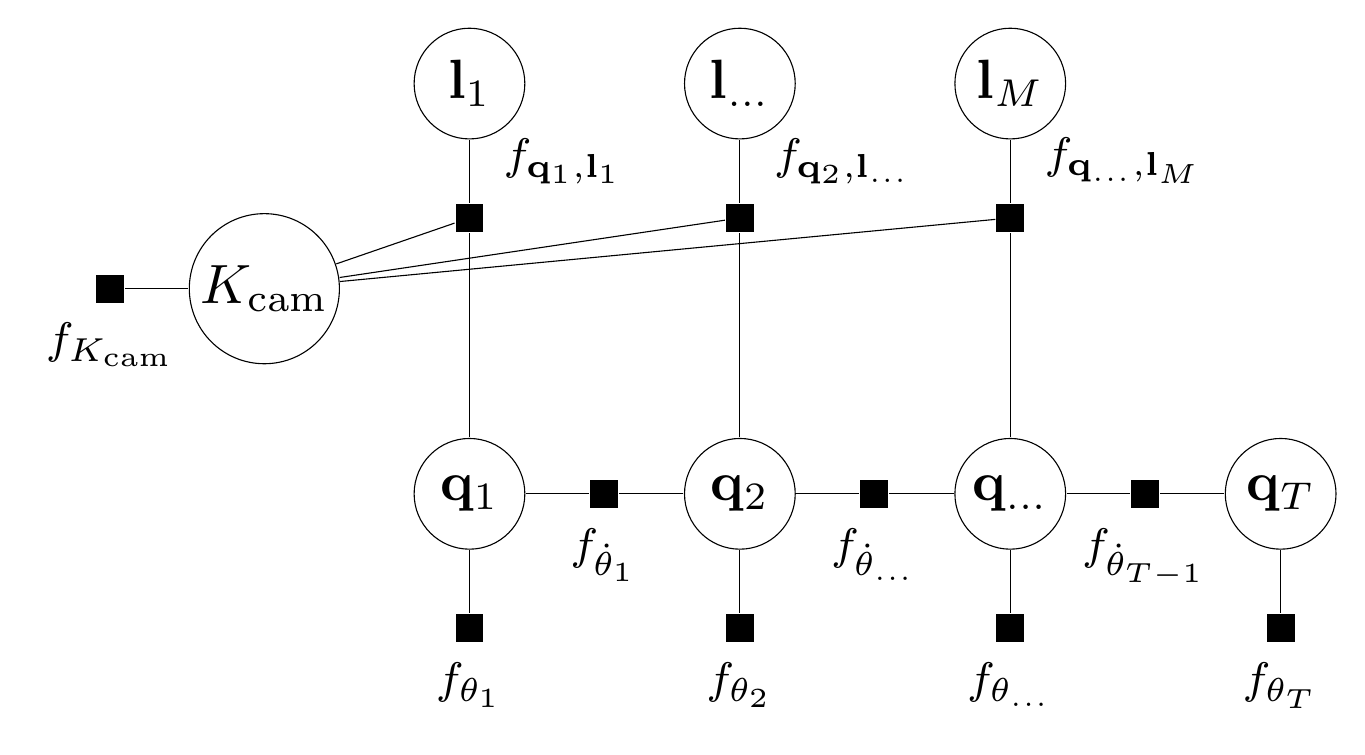
\begin{tikzpicture}[x=2cm, y=2.0cm, every node/.style={scale=2.0}]
	\node[latent] (k0) {$\Extr$};
	\node[latent, below right = of k0] (q1) {$\config_1$};
	\node[latent, right=of q1] (q2) {$\config_2$};
	\node[latent, right=of q2] (qN) {$\config_{\ldots}$};
    \node[latent, right=of qN] (qT) {$\config_T$};
    \node[latent, above right=of k0] (l1) {$\landmark_1$};
    \node[latent, right=of l1] (lN) {$\landmark_{\ldots}$};
    \node[latent, right=of lN] (lM) {$\landmark_M$};
    \factor[below=of l1] {l1-f} {above right:$f_{\config_1, \landmark_1}$}{}{};
    \factor[below=of lN] {lN-f} {above right:$f_{\config_2, \landmark_{\ldots}}$}{}{};
    \factor[below=of lM] {lM-f} {above right:$f_{\config_{\ldots}, \landmark_M}$}{}{};
    \factor[below=of q1] {q1-f} {below:$f_{\enc_1}$}{}{};
    \factor[below=of q2] {q2-f} {below:$f_{\enc_2}$}{}{};
    \factor[below=of qN] {qN-f} {below:$f_{\enc_{\ldots}}$}{}{};
    \factor[below=of qT] {qT-f} {below:$f_{\enc_T}$}{}{};
    \factor[right=of q1] {q1q2-f} {below:$f_{\dot{\enc}_1}$}{}{};
    \factor[right=of q2] {q2qN-f} {below:$f_{\dot{\enc}_{\ldots}}$}{}{};
    \factor[right=of qN] {qNqT-f} {below:$f_{\dot{\enc}_{T - 1}}$}{}{};
    \factor[left=of k0]{k0-f}{below:$f_{\Extr}$}{}{};
    \factoredge{k0}{k0-f}{};
    \factoredge{q1}{q1-f}{};
	\factoredge{q2}{q2-f}{};
	\factoredge{qN}{qN-f}{};
	\factoredge{qT}{qT-f}{};
	\factoredge{q1}{q1q2-f}{};
    \factoredge{q2}{q1q2-f}{};
    \factoredge{qN}{q2qN-f}{};
    \factoredge{q2}{q2qN-f}{};
    \factoredge{qT}{qNqT-f}{};
    \factoredge{qN}{qNqT-f}{};
    \factoredge{q1}{l1-f}{};
    \factoredge{q2}{lN-f}{};
    \factoredge{qN}{lM-f}{};
    \factoredge{l1}{l1-f}{};
    \factoredge{lM}{lM-f}{};
    \factoredge{lN}{lN-f}{};
    \factoredge{k0}{l1-f}{};
    \factoredge{k0}{lN-f}{};
    \factoredge{k0}{lM-f}{};
\end{tikzpicture}
\caption{Graphical model of the SLAM system.}
\label{fig:graphical_model}
\end{figure}

Each time a camera at timestep $t$ observes landmark $i$, we have a factor $f_{\config_t, \landmark_i}$ that correlates together the cmaera calibration, robot configuration, and landmark position. For simplicity \figref{fig:graphical_model} shows only one landmark observation per timestep, but in fact there may be many landmarks observed. The joint encoders are connected to robot configurations by the factors $f_{\theta_t}$. Robot configurations are themselves correlated over time by the fators $f_{\dot{\enc}_{t-1}}$. 

In the coming sections, we will describe how each of these nodes and factors are expressed in practice.

\subsection{Landmark Observation Factors}

\begin{figure}
\centering
\begin{tikzpicture}
  	\node[anchor=south west,inner sep=0] (image) at (0,0) {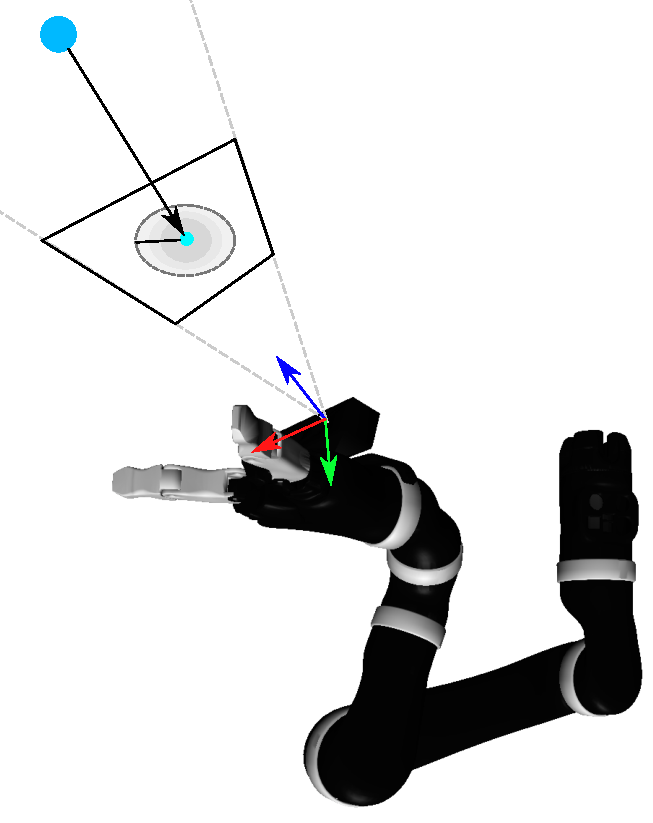
\includegraphics[width=0.75\textwidth]{img/graph_slam/projection_factor.pdf}};
  	\begin{scope}[x={(image.south east)},y={(image.north west)}]%
		%\draw[help lines,xstep=.1,ystep=.1] (0,0) grid (1,1); 
	    %\foreach \x in {0,1,...,9} { \node [anchor=north] at (\x/10,0) {0.\x}; }
	    %\foreach \y in {0,1,...,9} { \node [anchor=east] at (0,\y/10) {0.\y}; }
	    \node at (0.31, 0.69) {\Large$\measurement_i$};
	    \node at (0.1, 0.9) {\Large$\landmark_i$};
	    \node at (0.26, 0.685) {\Large$\Sigma_{\measurement}$};
	    \node at (0.55, 0.55) {\Large$\Extr$};
	    \node at (0.41, 0.78) {\Large$\Image_t$};
	    \node at (0.2, 0.2) {\Large$\config_t \left\{ \rule{0pt}{20mm}\right.$};
    \end{scope} 
\end{tikzpicture} 
\caption{Landmark observation factor. The robot at configuration $\config_t$ observes landmark $\landmark_i$ in image $\Image_t$. The noise is on the reprojection of the landmark into the image.}
\end{figure} 

The factors $f_{\config_t, \landmark_i}$ of the graph (\figref{fig:graphical_model}) represent the posterior probability of the robot's configuration, camera extrinsics, and landmark position given observations of the landmark $i$ at time $t$.

\begin{equation} 
	f_{\config_t, \landmark_i} = \Prob\left( \measurement_{i, t} | \config_t, \landmark_i, \Extr\right)
\end{equation}

\noindent here, we model a measurement of landmark $\landmark_i$ in camera image $I_t$ as a 2D pixel coordinate $\measurement_{i, t}$. The 3D landmark positions $\landmark_i$ is projected onto the camera image using the projection function

\begin{equation}
	 F_{\Proj}\left(\config_t, \Extr, \landmark_i\right) = \Proj\left(\left(F(\config) \Extr \right)\inv\landmark_i\right) 
\end{equation}

\noindent the measurement $\measurement_{i, t}$ can be modeled as a random variable sampled from the distribution

\begin{equation}
	\measurement_{i, t} \sim F_{\Proj}\left(\config_t, \Extr, \landmark_i\right) + \mathcal{N}(\mu_\measurement, \Sigma_\measurement)
\end{equation}

\noindent where $\mu_\measurement, \Sigma_\measurement$ are the mean and variance of the reprojection noise, respectively. Therefore,

\begin{equation}
	\Prob\left( \measurement_{i, t} | \config_t, \landmark_i, \Extr\right) = \mathcal{N}_{\mu_\measurement, \Sigma_\measurement}\left(F_{\Proj}\left(\config_t, \Extr, \landmark_i\right) - \measurement_{i, t}\right)
\end{equation}

\subsection{Joint Encoder Factors}
The factors $f_{\enc_t}$ represent the posterior probability of the robot's configuration given the joint encoder measurements at time $t$. That is

\begin{equation}
	f_{\enc_t} = \Prob\left(\enc_t | \config_t\right)
\end{equation}

\noindent as in chapters \ref{chap:dense_external_tracking} and \ref{chap:dense_slam}, we assume that the joint encoders are random variables drawn from gaussian noise on the true configuration of the robot

\begin{equation}
	\enc_t \sim K_\enc\inv\left(\config_t + \mathcal{N}(\mu_\enc, \Sigma_\enc)\right)
\end{equation}

\noindent where $\mu_\enc, \Sigma_\enc$ are the mean and covariance of the joint angle noise, respectively, and $K_\enc$ is the static joint encoder calibration function (\sref{sec:encoders}). Therefore the posterior is

\begin{equation}
	\Prob\left(\enc_t | \config_t\right) = \mathcal{N}_{\mu_\enc, \Sigma_\enc}\left(\config_t - K_\enc(\enc_t)\right)
\end{equation}

To account for gear backlash (\sref{sec:encoders}), we add a small \textit{dead band} $\Delta_\enc$ so that configurations within $\Delta_\enc$ of the joint encoders are not penalized:

 \begin{align}
	\Prob\left(\enc_t | \config_t\right) &= \mathcal{N}_{\mu_\enc, \Sigma_\enc}\left(\delta(\config_t - K_\enc(\enc_t))\right) \\
	\delta(\config_t - K_\enc(\enc_t)) &= \colvec{3}{\max\left\big(0, \|\config_t[1] - K_\enc(\enc_t)[1]\| - \Delta_\enc\right\big)\text{sgn}\left(\config_t[1] - K_\enc(\enc_t)[1]\right)}{\vdots}{\max\left\big(0, \|\config_t[N] - K_\enc(\enc_t)[N]\| - \Delta_\enc\right\big)\text{sgn}\left(\config_t[N] - K_\enc(\enc_t)[N]\right)}
\end{align}

\noindent where $\text{sgn}$ is the sign function. The gear backlash term $\delta$ allows the joint angles of the robot to vary within the dead-band $\Delta_\enc$ without penalty.

\subsection{Robot Dynamics Factors}

The factors $f_{\dot{\enc}_{t- 1}}$ correlate the robot's joint angles given joint velocity measurements $\dot{\enc}_{t - 1}$. That is

\begin{equation}
	f_{\dot{\enc}_{t- 1}} = \Prob(\dot{\enc}_{t - 1} | \config_{t - 1}, \config_{t})
\end{equation}

\noindent we assume that the velocity measurements are random variables drawn from the true velocity of the robot's joints, which we approximate with finite differencing. That is

\begin{equation}
	\dot{\enc}_{t - 1} \sim \frac{\qvec_{t} - \qvec_{t - 1}}{\Delta t} + \mathcal{N}(\mu_{\dot{\theta}}, \Sigma_{\dot{\theta}})
\end{equation}

\noindent where $\delta t$ is the timestep between time $t$ and $t-1$, $\mu_{\dot{theta}}$ is the mean of the velocity noise, and $\Sigma_{\dot{\theta}}$ is its covariance. Therefore

\begin{equation}
	\Prob(\dot{\enc}_{t - 1} | \config_{t - 1}, \config_{t}) = \mathcal{N}_{\mu_{\dot{\theta}}, \Sigma_{\dot{\theta}}}\left(\dot{\enc}_{t - 1} - \frac{\qvec_{t} - \qvec_{t - 1}}{\Delta t}\right)
\end{equation} 

The dynamics factors smooth our estimate of the joint angle trajectory so that it is closer to physically feasible than if only joint encoder factors are used. In part, we do this because the joint encoder posterior is not really representative of the true system dynamics that cause the joint encoders to be inaccurate. The inaccuracy stems from unmodeled systematic error that depends in part on the robot's configuration and torques it is applying. Adding a factor to constrain the motion of the joints allows us to smoothly predict the joint encoder error without having to explicitly model the physical process that causes it.

\subsection{Extrinsic Prior}
The factor $f_{\Extr}$ describes the prior distribution for the camera extrinsics. This is simply

\begin{align}
	f_{\Extr} &= \Prob(\Extr) \\
		      &= \mathcal{N}_{\mu_{\Extr}, \Sigma_{\Extr}}(\Extr)
\end{align}

\noindent where $\mu_{\Extr}, \Sigma_{\Extr}$ are the mean and covariance of the extrinsic prior, respectively.

\section{SLAM Back-end System Implementation}
As the robot receives joint encoder measurements and observations of landmarks, we add nodes and factors to the graphical model, which is then jointly optimized to find a maximum likelihood estimate of all the unknown variables ($\config_1, \ldots \config_T$, $\landmark_1, \ldots, \landmark_M$ and $\Extr$) given all the measurements. We consider both batch and online solutions. 

For the batch solution, we use Levenberg-Marquadt. For the online solution, we use the Incremental Smoothing and Mapping 2 (iSAM2) algorithm \cite{Kaess12ijrr}. For an explanation of how these algorithms work, \sref{sec:graph_slam}. We use off-the-shelf implementations of these algorithms from the Georgia Tech Smoothing and Mapping (GTSAM) \cite{gtsam} library, and make use of the outlier-robust Cauchy estimator found in GTSAM. 

\section{Landmark Front-end System Implementation}
To acquire landmarks from the camera images, we consider two systems: one based on April \cite{olson2010tags} tags, and another based on natural image features using the Binary Robust Invariant Scalable Keypoint (BRISK)\cite{Leutenegger2011BRISK} features.

\subsection{April Tag Front-end Implementation}

April tags are fiducials designed for computer vision and augmented reality consisting of unique grid patterns. These tags can be detected easily in 2D images, and with a known intrinsic calibration and tag size, their poses relative to the sensor can be estimated. Using April tags, the landmark $\landmark_i$ is simply the 3D location of the top-left corner of the April tag with tag id $i$. The initial position estimate of $\landmark_i$ is given by the pose estimate returned by the April tags detector (which also reports the pixel locations of each of the tag's corners). 

\begin{figure}
	\centering
	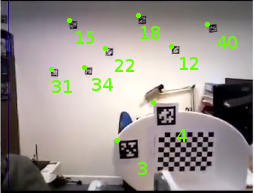
\includegraphics[width=0.5\textwidth]{img/graph_slam/apriltags}
	\caption{Detected April tags and their associated IDs.}
	\label{fig:april_tags}
\end{figure}

The April tags were used mainly to test the SLAM backend system without having to worrry about landmark association. Our system does not require the tags to detect and associate landmarks, but will use them when available.

\subsection{Natural Image Feature Front-end Implementation}

Acquiring and associating 3D landmarks from a series of natural images is somewhat more complicated than acquiring 3D landmarks from fiducials. First, we acquire a number of BRISK keypoints (\sref{sec:image_features}) $k_1, \ldots, k_n$ in the image $\Image_t$ roughly corresponding to corners and lines. Each keypoint is associated with a descriptor $d_1, \ldots, d_n$. 

\begin{figure}
	\centering
	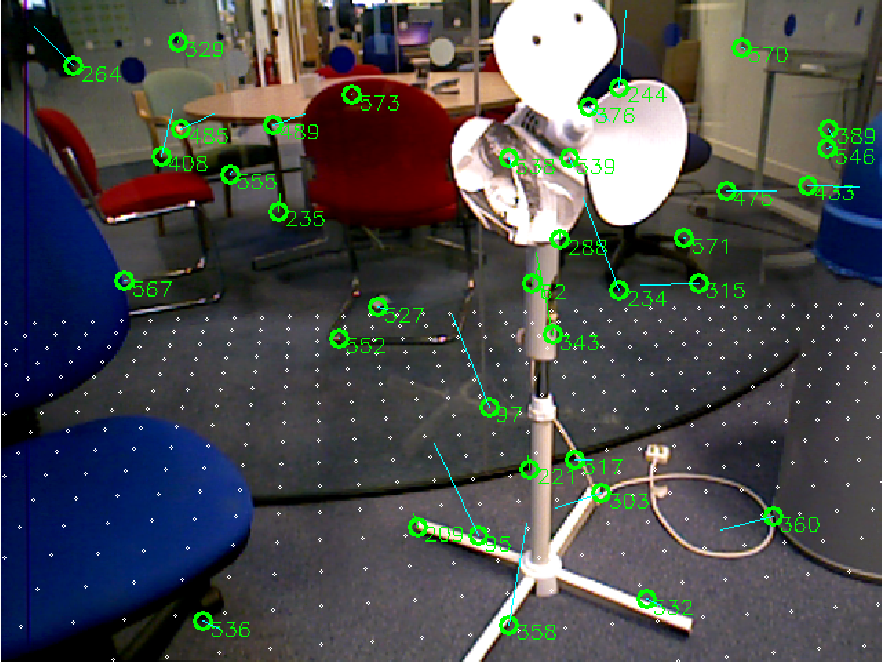
\includegraphics[width=0.5\textwidth]{img/graph_slam/brisk_features}
	\caption{Detected BRISK keypoints (green circles), their IDs, and reprojection error (blue lines). Also shown is the predicted ground plane (grey dots).}
	\label{fig:brisk_detections}
\end{figure}

Then, for each keypoint, we match it to the closest potential 3D landmark visible from the estimated robot configuration $\config_t$. We reject the match whenever the descriptor $d_i$'s Hamming distance to the existing landmark's last observed descriptor is too far, and accept it otherwise. Rejected matches get added to the pool of new potential 3D landmarks, but are not added to the facor graph until the following conditions are met:

\begin{itemize}
  \item The landmark has been matched to two or more camera images.
  \item There is a sufficient stereo baseline between camera observations of the landmark.
  \item The landmark can be successfully stereo-triangulated (\sref{sec:triangulation}) from its observations.
\end{itemize} 

The stereo triangulation system uses the current estimate of the robot's configuration to estimate the motion between frames. By conservatively eliminating outliers in this way, we minimize false-positive associations between image features. Still, some false-positive associations occur.

\section{Experiments}
\chapter{Discussion} \input{discussion}
  
\appendix
\chapter{Appendix} \section{Articulated Linkages and Robot Arms}
\label{sec:articulated_linkage}
An articulated linkage is a series of rigid bodies (called \textit{links}) connected by joints. Each joint has one or more degrees of freedom, and two associated links $A$ and $B$. A degree of freedom maps a value $q \in \ROne$ to a transformation $T^{A}_B(q) \in \SEThree$, which encodes the rigid transformation between links $A$ and $B$. A degree of freedom may correspond to a rotation, translation, or both. A degree of freedom may have limits $q_\text{min}, q_\text{max}$, that constrain its motion.

Robot arms are a special case of the kinematic linkage. Usually, robot arms are \textit{serial} linkages, meaning that the graph formed by links and joints is a tree, with the root fixed to the world, and allow for sensing and control of the degrees of freedom.

The set of degree of freedom values $\config = [q_1, \ldots, q_N]\trans$ is called the \textit{configuration} of the linkage, and is represented as a vector. The set of all possible configurations of the linkage $\config \in \Q$ is called the \textit{configuration space} \cite{Mason2001}. 


\subsection{Forward and Inverse Kinematics}
\label{sec:kinematics}
The configuration space of a linkage is related to its \textit{workspace} $\RThree$ by its \textit{forward} and \textit{inverse} kinematics. Using forward kinematics, any point on the robot's body $\xvec$ can be transformed into the workspace by the function $F_\xvec(\config) : \Q \to \RThree$. Forward kinematics encode a many-to-one relationship between a configuration and the points on the robot's body, and always has a solution. The forward kinematics can be computed merely be concatenating the link transformations together $F_\xvec(\config) = T^{N - 1}_{N}(q_N) \ldots T^{2}_3(q_2) T^{1}_2(q_1)$

The inverse of the kinematics function can also be defined, which for a point on the robot's body $\xvec$, returns the configuration which puts $\xvec$ at the desired location; $F_\xvec\inv(\xvec) : \RThree \to Q$. This is in general a one-to-many function, and may have no solution.

The first-order derivates of the kinematics functions can also be computed. The first-order derivative of the forward kinematics function $\J_\xvec = \frac{\partial}{\partial \config} F_\xvec \in \R^{3 \times N}$ is called the \textit{Jacobian} of the linkage. The inverse of the Jacobian $\J_\xvec\inv$ can also be defined. In general, the inverse of the Jacobian $\J_\xvec\inv$ describes the joint velocities required to move $\xvec$ at a specified linear velocity. If the robot has more or fewer degrees of freedom than $3$, the Moore-Penrose pseudoinverse of the Jacobian $\J_\xvec^{+}$ can be used instead. Through the \textit{principle of virtual work}, the transpose of the Jacobian $\J_\xvec\trans$ can be used to describe the instantaneous torques required to apply a linear force at $\xvec$.
  
\subsection{Encoders}
\label{sec:encoders}
The degrees of freedom of a robot can be measured by sensors called encoders. These include for example optical, resistive, current, and mechanical sensors. In general the output of an encoder $\enc$ can be used to estimate the value of its associated degree of freedom $q_\enc$ through an \textit{encoder calibration} function $q_\enc = K_e(\enc)$. For some encoders, the calibration function can be represented as a simple linear transformation. For other encoders, the calibration function must be more complex. 

Some robots have dynamic mechanisms (such as springs, gear trains or cables) between their encoders and associated degrees of freedom. These degrees of freedom may complciate the calibration function, adding dynamic factors such as the velocity and torque of the system.

\subsubsection{Gear Backlash}
\label{sec:encoders}
One particular dynamic effect of interest is \textit{gear backlash}, which occurs whenever a series of gears sits between the encoder and the robot's joint. This happens because tiny gaps between the gear teeth prevent the gears from being in contact all the time. Consequently, the joint or motor may rotate slightly without actually turning the gears. In principle, this limits the sensitivity of the joint encoder to small motions.

\section{Data Synchronization and Interpolation}

\section{Geometric Computer Vision}
\label{sec:vision}
\subsection{Pinhole Cameras}
\label{sec:cameras}
Optics describes the relation between geometric points in the world and their corresponding 2D image projections \cite{Hartley2004}. The simplest kind of optical system is a pinhole (\ie lensless) camera. A simple pinhole camera consists of a rigid transformation $T_\text{cam} \in \SEThree$, and a \textit{intrinsic matrix}

\begin{equation}
K = \left[ \begin{array}{cccc} 
             f_x & 0 & c_x & 0 \\
             0 &  f_y & c_y & 0\\ 
             0 &    0 &   0 & 1
    \end{array} \right]
\end{equation}

\noindent where $f_x, f_y$ are the focal lengths, and $c_x, c_y$ are the image center. The intrinsic matrix can be used to turn pixel coordinates $\pixel \in \Imagespace$ into homogenous intrinsic coordinates $\pixel'$ by the equation:

\begin{equation} 
	\pixel' = K \colvec{2}{\pixel}{1}
\end{equation}

\noindent the homogenous intrinsic coordinates $p'$ at depth $z$ can be converted into a point in the world $\xvec$ using the projection function

\begin{equation}
 \xvec = \Proj\left(\pixel', z\right) = T_\text{cam} \colvec{3}{\pixel'_x z}{\pixel'_y z}{z}
\end{equation}

\subsection{Stereo Triangulation}
\label{sec:triangulation}
\subsection{RGB-D Cameras}
\label{sec:rgbd} 
RGB-D cameras (or \textit{depth cameras}) are sensors which provide both color images and depth images. Projective depth cameras, such as the Microsoft \textit{Kinect}, Asus \textit{Xtion} or Occipital \textit{Structure} sensor work by projecting an infrared pattern onto the scene. By measuring the deformation of the pattern as viewed by an infrared camera, an estimate for depth can be achieved with stereo triangulation. This depth estimate is limited by the stereo baseline of the infrared camera and projector, and usually falls between 0.4 and 3 meters. 

The \textit{point cloud} of a depth image is defined as all of the valid pixels in the depth image unprojected into the scene using the depth camera's intrinsics.

\section{Simultaneous Localization and Mapping (SLAM)}
\label{sec:SLAM}
\subsection{Dense SLAM}
\label{sec:dense_slam}
\subsection{Graph-based SLAM}
\label{sec:graph_slam}

\section{2D Image Features and Association}
\label{sec:image_features}
\subsection{BRISK Image Features}
\subsection{Landmark Association}

\backmatter

%\renewcommand{\baselinestretch}{1.0}\normalsize

% By default \bibsection is \chapter*, but we really want this to show
% up in the table of contents and pdf bookmarks.
\renewcommand{\bibsection}{\chapter{\bibname}}
%\newcommand{\bibpreamble}{This text goes between the ``Bibliography''
%  header and the actual list of references}
\bibliographystyle{plainnat}
\bibliography{references.bib} %your bib file

\end{document}